%TC:ignore
\documentclass{article}
\usepackage{caption}
\usepackage{xcolor, colortbl}
\definecolor{RED}{HTML}{EB6231}
\definecolor{BLUE}{HTML}{5D80B4}
\definecolor{LIGHTGREY}{gray}{0.9}
\definecolor{BLUELINK}{HTML}{0645AD}
\definecolor{DARKBLUELINK}{HTML}{0B0080}
\PassOptionsToPackage{hyphens}{url}
\usepackage[colorlinks=false]{hyperref}
% for linking between references, figures, TOC, etc in the pdf document
\hypersetup{colorlinks,
    linkcolor=DARKBLUELINK,
    anchorcolor=DARKBLUELINK,
    citecolor=DARKBLUELINK,
    filecolor=DARKBLUELINK,
    menucolor=DARKBLUELINK,
    urlcolor=BLUELINK
} % Color citation links in purple
\PassOptionsToPackage{unicode}{hyperref}
\PassOptionsToPackage{naturalnames}{hyperref}

\usepackage[backend=biber,eprint=false,isbn=false,url=false,intitle=true,style=nature,date=year]{biblatex}
\addbibresource{codon_models.bib}

\usepackage{bbm}
\usepackage[margin=50pt]{geometry}
\usepackage{amssymb,amsfonts,amsmath,amsthm,mathtools}
\usepackage{lmodern}
\usepackage{bm,bbold}
\usepackage{verbatim}
\usepackage{float}
\usepackage{listings, enumerate, enumitem}
\usepackage[export]{adjustbox}
\usepackage{tabu}
\usepackage{longtable}
\tabulinesep=0.6mm
\newcommand\cellwidth{\TX@col@width}
\usepackage{hhline}
\setlength{\arrayrulewidth}{1.2pt}
\usepackage{multicol,multirow,array}
\usepackage{etoolbox}
\AtBeginEnvironment{tabu}{\footnotesize}
\usepackage{booktabs}
\usepackage{makecell}
\usepackage{orcidlink}
\usepackage{graphicx}
\usepackage{blkarray}
\usepackage{pgf,tikz}
\usetikzlibrary{shapes,arrows,backgrounds,fit,positioning,arrows,automata,calc}
\tikzset{res/.style={ellipse,draw,minimum height=1.0cm,minimum width=0.8cm}}
\tikzset{literal/.style={rectangle,draw,minimum height=0.5cm,minimum width=0.8cm,text width = 1.2 cm, align = center}}

\pdfinclusioncopyfonts=1

\renewcommand{\baselinestretch}{1.5}
\renewcommand{\arraystretch}{0.6}
\frenchspacing

\renewcommand{\thetable}{S\arabic{table}}
\renewcommand{\thefigure}{S\arabic{figure}}
\renewcommand{\theequation}{S.\arabic{equation}}

\newcommand{\UniDimArray}[1]{\bm{#1}}
\newcommand{\BiDimArray}[1]{\bm{#1}}

\newcommand{\der}{\text{d}}
\newcommand{\e}{\text{e}}
\newcommand{\Ne}{N_{\text{e}}}
\newcommand{\proba}{\mathbb{P}}
\newcommand{\pfix}{\proba_{\text{fix}}}
\newcommand{\dn}{d_N}
\newcommand{\ds}{d_S}
\newcommand{\dnds}{\dn / \ds}
\newcommand{\Sphy}{S_{0}}
\newcommand{\SphyMean}{\overline{\Sphy}}
\newcommand{\SphyDel}{\mathcal{D}_0}
\newcommand{\SphyNeu}{\mathcal{N}_0}
\newcommand{\SphyBen}{\mathcal{B}_0}
\newcommand{\Sphyclass}{x}
\newcommand{\SphyclassAlt}{y}
\newcommand{\given}{\mid}
\newcommand{\Spop}{S}
\newcommand{\SpopDel}{\mathcal{D}}
\newcommand{\SpopNeu}{\mathcal{N}}
\newcommand{\SpopBen}{\mathcal{B}}
\newcommand{\ProbaPopDel}{\proba [ \SpopDel]}
\newcommand{\ProbaPopNeu}{\proba [ \SpopNeu ]}
\newcommand{\ProbaPopBen}{\proba [ \SpopBen ]}
\newcommand{\AdvMean}{\beta_b}
\newcommand{\DelMean}{\beta_d}
\newcommand{\thetaSyn}{\theta_{\text{S}}}
\newcommand{\pvalue}{p\text{-value}}

% Model
\newcommand{\submatrix}{q}
\newcommand{\Submatrix}{\BiDimArray{\submatrix}}
\newcommand{\probmatrix}{P}
\newcommand{\Probmatrix}{\BiDimArray{\probmatrix}}
\newcommand{\fit}{F}
\newcommand{\Fit}{\UniDimArray{\fit}}
\newcommand{\indice}{l}
\newcommand{\indiceexp}{^{(\indice)}}
\newcommand{\ci}{{a}}
\newcommand{\cj}{{b}}
\newcommand{\itoj}{\ci \mapsto \cj}
\newcommand{\nuc}{\mathcal{M}}
\newcommand{\fiti}{\fit_{\ci}}
\newcommand{\fitj}{\fit_{\cj}}
\newcommand{\mutmatrix}{R}
\newcommand{\Mutmatrix}{\BiDimArray{\mutmatrix}}
\newcommand{\exchan}{\rho}
\newcommand{\Exchan}{\UniDimArray{\exchan}}
\newcommand{\mutequi}{\sigma}
\newcommand{\Mutequi}{\UniDimArray{\mutequi}}
\newcommand{\Tree}{\mathcal{T}}
\newcommand{\branch}{\text{j}}
\newcommand{\branchexp}{^{(\branch)}}
\newcommand{\branchlength}{l}
% Alignment
\newcommand{\data}{D}
\newcommand{\Data}{\BiDimArray{\data}}
\newcommand{\site}{\text{i}}
\newcommand{\Nsite}{\text{N}}
\newcommand{\siteexp}{^{(\site)}}
\newcommand{\Setsite}{\site \in \{1, \hdots, \Nsite\} }
\newcommand{\branchsiteexp}{^{(\branch, \site)}}
% Categories
\newcommand{\cat}{\text{k}}
\newcommand{\Ncat}{\text{K}}
\newcommand{\catexp}{^{(\cat)}}
\newcommand{\catInterval}{\{1, \hdots, \Ncat\}}
\newcommand{\Setcat}{\cat \in \catInterval }
\newcommand{\branchcatexp}{^{(\branch, \cat)}}
\newcommand{\profile}{\phi}
\newcommand{\Profile}{\UniDimArray{\profile}}
\newcommand{\concentrationProfile}{\alpha}
\newcommand{\centerProfile}{\UniDimArray{\gamma}}
\newcommand{\catVar}{\kappa}
\newcommand{\catsite}{\catVar\left(\site\right)}
\newcommand{\catmultivar}{m}
\newcommand{\catMultiVar}{\UniDimArray{\catmultivar}}
\newcommand{\stickbreaking}{\theta}
\newcommand{\StickBreaking}{\UniDimArray{\stickbreaking}}
\newcommand{\stick}{\psi}
\newcommand{\stickbreakinghyper}{\beta}
\newcommand{\Multivariate}{\UniDimArray{Z}}
\newcommand{\subhistory}{\mathcal{H}}

\title{\textbf{Mammalian protein-coding genes exhibit widespread beneficial mutations that are not adaptive}}

\author{
    \large
    \textbf{T. {Latrille}$^{1\dag}$\orcidlink{0000-0002-9643-4668}, J. {Joseph}$^{2\dag}$\orcidlink{0009-0002-1312-9930}, D.~A. {Hartasánchez}$^{1}$\orcidlink{0000-0003-2596-6883}, N. {Salamin}$^{1}$\orcidlink{0000-0002-3963-4954}}\\
    \scriptsize $^{1}$Department of Computational Biology, Université de Lausanne, Lausanne, Switzerland\\
    \scriptsize $^{2}$Laboratoire de Biométrie et Biologie Evolutive, UMR5558, Université Lyon 1, Villeurbanne, France \\
    \scriptsize $^{\dag}$These authors contributed equally to this work\\
    \normalsize \texttt{\href{mailto:thibault.latrille@ens-lyon.org}{thibault.latrille@ens-lyon.org}} \\
}


\date{}

\begin{document}
    \maketitle
    \part*{Supplementary materials}
    \tableofcontents
    \clearpage

    \section{Mutation-selection codon models}\label{sec:mutsel}

    \subsection{Prior distributions and parameters of the model}\label{subsec:priors}

    The parameterization of the models is described as a Bayesian hierarchical model, including the prior distributions and the parameters of the model.
    This hierarchical model is formally represented as directed acyclic graph of dependencies between variables, depicted below.
    Nodes of the directed acyclic graph are the variables, and edges are the functions.
    Hyper-parameters are depicted in {\color{RED}{red}} circles, random variables in {\color{BLUE}{blue}} circles, and transformed variables in black.
            {\color{BLUE}{Blue}} dashed line denotes a drawing from a random distribution, and black solid lines denote a function.
    All the nodes pointing toward a given node (upstream) are its dependencies which determines its distribution.
    The other way around, following the arrows in the DAG (downstream), simple {prior} distributions are combined together to form more complex joint {prior} distribution which ultimately defines the {prior} distribution of the model.

    \begin{center}
        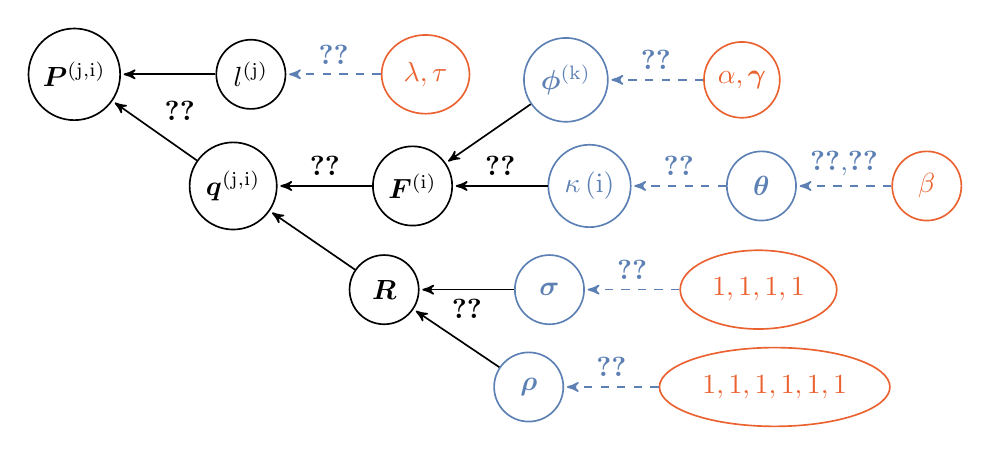
\begin{tikzpicture}[->,>=stealth',shorten >=1pt,auto,node distance=0.6cm and 1.2cm,semithick]
            \tikzstyle{every state}=[]

            \node[state] (P) {$\Probmatrix\branchsiteexp$};
            \node[state] (Q) [below right=of P] {$\Submatrix\branchsiteexp$};
            \node[state] (R) [below right=of Q] {$\Mutmatrix$};
            \node[state] (BL) [right=of P] {$\branchlength\branchexp$};
            \node[res] (BLH) [RED, right=of BL] {$ \lambda, \tau $};
            \node[state] (f) [right=of Q] {$\Fit\siteexp $};
            \node[state] (Ex) [BLUE, below right=of R] {$\Exchan$};
            \node[state] (Equi) [BLUE, right=of R] {$\Mutequi$};
            \node[state] (Base) [BLUE, above right=of f] {$\Profile\catexp$};
            \node[state] (cat) [BLUE, right=of f] {$\catsite$};
            \node[res] (ExH) [RED, right=of Ex] {$1,1,1,1,1,1$};
            \node[res] (EquiH) [RED, right=of Equi] {$1,1,1,1$};
            \node[state] (baseH) [RED, right=of Base] {$\concentrationProfile, \centerProfile $};
            \node[state] (sb) [BLUE, right=of cat] {$\StickBreaking$};
            \node[state] (sbH) [RED, right=of sb] {$\stickbreakinghyper$};

            \path
            (Q) edge [black] node [above right] {\ref{eq:Probmatrix}} (P)
            (BL) edge [black] node [] {} (P)
            (R) edge [black] node {} (Q)
            (f) edge [black] node [above] {\ref{eq:subrates}} (Q)
            (Ex) edge [black] node [] {} (R)
            (Equi) edge [black] node [below] {\ref{eq:gtr-mutrates}} (R)
            (Base) edge [black] node {} (f)
            (cat) edge [black] node [above] {\ref{eq:sitefitness}} (f)
            (BLH) edge [dashed, BLUE] node [above] {\ref{eq:branchlength}} (BL)
            (ExH) edge [dashed, BLUE] node [above] {\ref{eq:DistribExchan}} (Ex)
            (EquiH) edge [dashed, BLUE] node [above] {\ref{eq:DistribMutequi}} (Equi)
            (baseH) edge [dashed, BLUE] node [above] {\ref{eq:DistribBase}} (Base)
            (sb) edge [dashed, BLUE] node [above] {\ref{eq:DistribMultinomial}} (cat)
            (sbH) edge [dashed, BLUE] node [above] {\ref{eq:DistribStickBreaking},\ref{eq:Beta}} (sb);
        \end{tikzpicture}
    \end{center}

    \subsection{Nucleotide mutation rates}
    The generalized time-reversible (GTR) nucleotide mutation rate matrix $\Mutmatrix$ is a function of the nucleotide frequencies $\Mutequi$ and the symmetric exchangeability rates $\Exchan$~\cite{tavare_probabilistic_1986}.
    $\Mutequi = (\mutequi_A , \mutequi_C , \mutequi_G , \mutequi_T)$ is the equilibrium base frequency vector, giving the frequency at which each base occurs at each site.
    $\Exchan = \left( \exchan_{AC}, \exchan_{AG}, \exchan_{AT}, \exchan_{CG}, \exchan_{CT}, \exchan_{GT}\right)$ is the vector of exchangeabilities between nucleotides.
    Altogether, the rate matrix is:
    \begin{equation}
        \label{eq:gtr-mutrates}
        \Mutmatrix =
        \begin{blockarray}{ccccc}
            & A & C & G & T \\
            \begin{block}{c(cccc)}
                A & - & {\exchan_{AC}\mutequi_C} & {\exchan_{AG}\mutequi_G} & {\exchan_{AT}\mutequi_T} \\
                C & {\exchan_{AC}\mutequi_A} &                        - & {\exchan_{CG}\mutequi_G} & {\exchan_{CT}\mutequi_T} \\
                G & {\exchan_{AG}\mutequi_A} & {\exchan_{CG}\mutequi_C} &                        - & {\exchan_{GT}\mutequi_T} \\
                T & {\exchan_{AT}\mutequi_A} & {\exchan_{CT}\mutequi_C} & {\exchan_{GT}\mutequi_G} & - \\
            \end{block}
        \end{blockarray}
    \end{equation}
    By definition, the sum of the entries in each row of the nucleotide rate matrix $\Mutmatrix$ is equal to $0$, giving the diagonal entries:
    \begin{equation}
        \mutmatrix_{a,a} = - \sum\limits_{ b \neq a, b \in \{A, C, G, T\} } \mutmatrix_{a,b}
    \end{equation}
    The {prior} on the exchangeabilities $\Exchan$ is a uniform Dirichlet distribution of dimension $6$:
    \begin{equation}
        \label{eq:DistribExchan}
        \Exchan \sim \text{Dir}\left( 1,1,1,1,1,1 \right).
    \end{equation}
    The {prior} on the equilibrium base frequencies $\Mutequi$ is a uniform Dirichlet distribution of dimension $4$:
    \begin{equation}
        \label{eq:DistribMutequi}
        \Mutequi \sim \text{Dir}\left( 1,1,1,1 \right)
    \end{equation}
    The general time-reversible nucleotide matrix is normalized with a total flow of $1$:
    \begin{equation}
        \sum\limits_{a \in \{A, C, G, T\}} - \mutequi_a \mutmatrix_{a,a} = 1,
    \end{equation}
    such that we expect $1$ {substitution} per unit of branch length.

    \subsection{Site-specific amino-acid fitness profiles}
    \label{sec:profiles}
    Site-specific amino-acid fitness profiles are assumed i.i.d. from a mixture model, itself endowed with a truncated Dirichlet process prior.
    Specifically, the mixture has $\Ncat$ components ($\Ncat = 30$ by default).
    The prior on component weights~($\StickBreaking$) is modeled using a stick-breaking process, truncated at $\Ncat$ and of parameter $\stickbreakinghyper=1$:
    \begin{align}
        \label{eq:DistribStickBreaking}
        \begin{split}
            & \StickBreaking \sim \text{StickBreaking}\left( \Ncat, \stickbreakinghyper \right)\\
            \iff & \stickbreaking_{\cat} = \stick_{\cat}\cdot \prod _{{\indice=1}}^{{\cat-1}}\left(1-\stick_{\indice}\right),\ \Setcat,
        \end{split}
    \end{align}
    where $\stick_{\cat}$ are i.i.d. from a beta distribution
    \begin{equation}
        \label{eq:Beta}
        \stick_{\cat} \sim \text{Beta}\left( 1, \stickbreakinghyper \right),\ \Setcat.
    \end{equation}
    Of note, the weights decrease geometrically in expectation, at rate $\stickbreakinghyper$, such that lower values of $\stickbreakinghyper$ induce more heterogeneous distributions of weights.

    Each component of the mixture defines a 20-dimensional fitness profile $\Profile\catexp$ (summing to $1$), for $ \Setcat$.
    These fitness profiles are i.i.d. from a Dirichlet of center $\centerProfile=1$ and concentration $\concentrationProfile=1$:
    \begin{equation}
        \label{eq:DistribBase}
        \Profile\catexp \sim \text{Dir}\left( \centerProfile,\ \concentrationProfile \right),\ \Setcat.
    \end{equation}

    Site allocations to the mixture components $\catsite \in \catInterval $, for $\Setsite$ running over the $\Nsite$ sites of the alignment, are i.i.d. multinomial of parameter $\StickBreaking$:
    \begin{align}
        \label{eq:DistribMultinomial}
        \catMultiVar \sim \text{Multinomial}\left( \StickBreaking \right), \\
        \text{ where } \catmultivar_{\cat} = \sum_{\Setsite} \mathbbm{1}_{\catsite = \cat}
    \end{align}

    For a given parameter configuration for the mixture, the scaled fitness $\Fit\siteexp$ at site $\site$, are obtained by taking the logarithm of fitness assigned to this site:
    \begin{equation}
        \label{eq:sitefitness}
        \Fit\siteexp = \ln \left( \Profile^{\left( \catsite \right)} \right),\ \Setsite.
    \end{equation}

    \subsection{Branch length}
    The topology of the rooted phylogenetic tree is supposed to be known and is not estimated by the model.
    The branch lengths $\branchlength\branchexp$ are defined as the expected number of {neutral} substitutions per {DNA} site along a branch, each from a Gamma distribution of mean $\lambda=0.1$ and scale $\tau=1$:
    \begin{equation}
        \label{eq:branchlength}
        \branchlength\branchexp \sim \text{Gamma}\left( \lambda, \tau \right).
    \end{equation}

    \subsection{Codon substitution rates}

    The mutation rate between codons $\ci$ and $\cj$, denoted $\mu_{\itoj}$ depends on the underlying nucleotide change between the codons.
    First, if codons $\ci$ and $\cj$ are not nearest-neighbours, $\mu_{\itoj}$ is equal to $0$.
    Second, if codons $\ci$ and $\cj$ are only one mutation away, $\mu_{\itoj}$ is given by the underlying nucleotide relative rate~(${\mutmatrix_{\itoj}}$).

    For a given site $\site$, the {codon} {substitution} rate matrix $\Submatrix\siteexp$ is given by:
    \begin{equation}
        \label{eq:subrates}
        \begin{dcases}
            \submatrix\siteexp_{\itoj} = 0\text{ if codons $\ci$ and $\cj$ are not nearest-neighbors,} \\
            \submatrix\siteexp_{\itoj} = \mu_{\itoj}\text{ if codons $\ci$ and $\cj$ are {synonymous},} \\
            \submatrix\siteexp_{\itoj} = \mu_{\itoj} \dfrac{ \fitj\siteexp - \fiti\siteexp}{{1 - \e^{\fiti\siteexp - \fitj\siteexp} }} \text{ if $\ci$ and $\cj$ are non-synonymous,}\\
            \submatrix\siteexp_{\ci, \ci} = - \sum\limits_{ \cj \neq \ci, \cj=1}^{61} \submatrix\siteexp_{\itoj}.
        \end{dcases}
    \end{equation}
    Together, the probability of transition between codons for a given branch $\branch$ and site $\site$ is:
    \begin{equation}
        \label{eq:Probmatrix}
        \Probmatrix\branchsiteexp = \e^{\branchlength\branchexp \Submatrix\siteexp},
    \end{equation}
    which are the matrices necessary to compute the {likelihood} of the data ($\data$) given the parameters of the model using the pruning algorithm.

    \subsection{Bayesian implementation}
    \label{sec:Bayesian}
    Bayesian inference was conducted using Markov Chain Monte Carlo (MCMC).
    Most phylogenetic {MCMC} samplers target the distribution over the model parameters given the sequence alignment, which means that they have to repeatedly invoke the pruning algorithm to recalculate the {likelihood} which is most often the limiting step of the {MCMC}.
    An alternative, which is used here, is to do the {MCMC} conditionally on the detailed {substitution} history $\subhistory$, thus doing the {MCMC} over the augmented configuration~($\subhistory$, $\data$), under the target distribution obtained by combining the mapping-based {likelihood} with the {prior} over model parameters.
    The key idea that makes this strategy efficient is that the mapping-based {likelihood} depends on compact summary statistics of $\subhistory$, leading to very fast evaluation of the {likelihood}.
    On the other hand, this requires to implement more complex {MCMC} procedures that have to alternate between:
    \begin{enumerate}
        \item sampling $\subhistory$ conditionally on the data and the current parameter configuration.
        \item re-sampling the parameters conditionally on $\subhistory$.
    \end{enumerate}

    To implement the mapping-based {MCMC} sampling strategy, we first sample the detailed {substitution} history $\subhistory$ for all sites along the tree.
    Several methods exist for doing this~\cite{nielsen_mapping_2002,rodrigue_uniformization_2008}, which are used here in combination (first trying the accept-reject method of Nielsen, then switching to the uniformization approach of Rodrigue \textit{et al} if the first round has failed).

    Then, we write down the probability of $\subhistory$ given the parameters, and finally, we collect all factors that depend on some parameter of interest and make some simplifications.
    This ultimately leads to relatively compact sufficient statistics allowing for fast numerical evaluation of the likelihood~\cite{irvahn_phylogenetic_2014,davydov_state_2017}.

    \subsection{BayesCode software}\label{subsec:bayescode}
    In \textit{BayesCode} (\href{https://github.com/ThibaultLatrille/BayesCode}{github.com/ThibaultLatrille/BayesCode}, v1.3.1), we ran the mutation-selection codon models \textit{mutselomega} for 2000 points of MCMC with the options:
    \begin{scriptsize}
        \begin{verbatim}
 mutselomega ---omegashift 0.0 --ncat 30 -a my_alignment.phy -t my_tree.newick -u 2000 my_genename
        \end{verbatim}
    \end{scriptsize}
    The collection of site-specific fitness profiles ($\UniDimArray{F^{(i)}}, \forall i$) are then obtained by running \textit{readmutselomega}, reading 1000 points of MCMC (first 1000 are considered as burn-in) with the options:
    \begin{scriptsize}
        \begin{verbatim}
 readmutselomega --every 1 --until 2000 --burnin 1000 --ss my_genename
        \end{verbatim}
    \end{scriptsize}
    The gene-specific $4 \times 4$ nucleotide mutation rate matrix ($\UniDimArray{\mu}$) is also obtained by running \textit{readmutselomega}, reading 1000 points of MCMC (first 1000 are considered as burn-in) with the options:
    \begin{scriptsize}
        \begin{verbatim}
 readmutselomega --every 1 --until 2000 --burnin 1000 --nuc my_genename
        \end{verbatim}
    \end{scriptsize}

    \newpage

    \section{Beneficial mutations in the terminal lineages and populations}\label{sec:beneficial-mutations}

    \subsection{Summary tables}\label{subsec:summary-table-mutsel}

    \subsubsection{Probability of mutations and substitutions to be $\SphyDel$, $\SphyNeu$ or $\SphyBen$}
    \begin{center}
        \captionof{table}{Probability of mutations and substitutions to be $\SphyDel$, $\SphyNeu$ or $\SphyBen$.}
        \scriptsize
        \begin{longtable*}{|l|l|r|r|r|r|r|r|}
            \toprule
            Population &             Species & $\proba[ \SphyDel ]$ & $\proba[ \SphyNeu ]$ & $\proba[ \SphyBen ]$ & $\proba_{div}[ \SphyDel ]$ & $\proba_{div}[ \SphyNeu ]$ & $\proba_{div}[ \SphyBen ]$ \\
            \midrule
            \endhead
            \midrule
            \multicolumn{8}{r}{{Continued on next page}} \\
            \midrule
            \endfoot

            \bottomrule
            \endlastfoot
            \rowcolor{LIGHTGREY} Equus c. & Equus caballus & $ 0.923$ & $ 0.065$ & $ 0.012$ & $ 0.462$ & $ 0.419$ & $ 0.118$ \\
            Iran & Bos taurus & $ 0.924$ & $ 0.065$ & $ 0.011$ & $ 0.515$ & $ 0.362$ & $ 0.123$ \\
            Uganda & Bos taurus & $ 0.924$ & $ 0.065$ & $ 0.011$ & $ 0.514$ & $ 0.361$ & $ 0.125$ \\
            \rowcolor{LIGHTGREY} Australia & Capra hircus & $ 0.923$ & $ 0.066$ & $ 0.011$ & $ 0.494$ & $ 0.386$ & $ 0.121$ \\
            \rowcolor{LIGHTGREY} France & Capra hircus & $ 0.923$ & $ 0.066$ & $ 0.011$ & $ 0.494$ & $ 0.386$ & $ 0.120$ \\
            \rowcolor{LIGHTGREY} Iran (C. aegagrus) & Capra hircus & $ 0.923$ & $ 0.066$ & $ 0.011$ & $ 0.493$ & $ 0.386$ & $ 0.120$ \\
            \rowcolor{LIGHTGREY} Iran & Capra hircus & $ 0.923$ & $ 0.066$ & $ 0.011$ & $ 0.492$ & $ 0.387$ & $ 0.121$ \\
            \rowcolor{LIGHTGREY} Italy & Capra hircus & $ 0.923$ & $ 0.066$ & $ 0.011$ & $ 0.494$ & $ 0.386$ & $ 0.120$ \\
            \rowcolor{LIGHTGREY} Morocco & Capra hircus & $ 0.923$ & $ 0.066$ & $ 0.011$ & $ 0.491$ & $ 0.387$ & $ 0.122$ \\
            Iran & Ovis aries & $ 0.922$ & $ 0.067$ & $ 0.012$ & $ 0.568$ & $ 0.323$ & $ 0.109$ \\
            Iran (O. orientalis) & Ovis aries & $ 0.922$ & $ 0.067$ & $ 0.011$ & $ 0.573$ & $ 0.320$ & $ 0.108$ \\
            Iran (O. vignei) & Ovis aries & $ 0.922$ & $ 0.067$ & $ 0.012$ & $ 0.567$ & $ 0.325$ & $ 0.109$ \\
            Various & Ovis aries & $ 0.922$ & $ 0.067$ & $ 0.011$ & $ 0.572$ & $ 0.321$ & $ 0.107$ \\
            Morocco & Ovis aries & $ 0.922$ & $ 0.067$ & $ 0.012$ & $ 0.570$ & $ 0.321$ & $ 0.108$ \\
            \rowcolor{LIGHTGREY} Barbados & Chlorocebus sabaeus & $ 0.926$ & $ 0.065$ & $ 0.009$ & $ 0.485$ & $ 0.393$ & $ 0.122$ \\
            \rowcolor{LIGHTGREY} Central Afr. Rep. & Chlorocebus sabaeus & $ 0.926$ & $ 0.065$ & $ 0.009$ & $ 0.485$ & $ 0.391$ & $ 0.124$ \\
            \rowcolor{LIGHTGREY} Ethiopia & Chlorocebus sabaeus & $ 0.926$ & $ 0.065$ & $ 0.009$ & $ 0.484$ & $ 0.393$ & $ 0.124$ \\
            \rowcolor{LIGHTGREY} Gambia & Chlorocebus sabaeus & $ 0.926$ & $ 0.065$ & $ 0.009$ & $ 0.483$ & $ 0.394$ & $ 0.123$ \\
            \rowcolor{LIGHTGREY} Kenya & Chlorocebus sabaeus & $ 0.926$ & $ 0.065$ & $ 0.009$ & $ 0.485$ & $ 0.392$ & $ 0.123$ \\
            \rowcolor{LIGHTGREY} Nevis & Chlorocebus sabaeus & $ 0.926$ & $ 0.065$ & $ 0.009$ & $ 0.484$ & $ 0.393$ & $ 0.123$ \\
            \rowcolor{LIGHTGREY} South Africa & Chlorocebus sabaeus & $ 0.926$ & $ 0.065$ & $ 0.009$ & $ 0.480$ & $ 0.394$ & $ 0.125$ \\
            \rowcolor{LIGHTGREY} Saint Kitts & Chlorocebus sabaeus & $ 0.926$ & $ 0.065$ & $ 0.009$ & $ 0.483$ & $ 0.394$ & $ 0.123$ \\
            \rowcolor{LIGHTGREY} Zambia & Chlorocebus sabaeus & $ 0.926$ & $ 0.065$ & $ 0.009$ & $ 0.485$ & $ 0.393$ & $ 0.123$ \\
            African & Homo sapiens & $ 0.925$ & $ 0.065$ & $ 0.010$ & $ 0.561$ & $ 0.341$ & $ 0.099$ \\
            Admixed American & Homo sapiens & $ 0.925$ & $ 0.065$ & $ 0.010$ & $ 0.561$ & $ 0.340$ & $ 0.099$ \\
            East Asian & Homo sapiens & $ 0.925$ & $ 0.065$ & $ 0.010$ & $ 0.560$ & $ 0.341$ & $ 0.098$ \\
            European & Homo sapiens & $ 0.925$ & $ 0.065$ & $ 0.010$ & $ 0.562$ & $ 0.340$ & $ 0.098$ \\
            South Asian & Homo sapiens & $ 0.925$ & $ 0.065$ & $ 0.010$ & $ 0.561$ & $ 0.341$ & $ 0.099$ \\
        \end{longtable*}
    \end{center}
    \begin{itemize}
        \item $\proba [ \SphyDel ]$ (eq.~5) is the probability for a new mutation to be a deleterious.
        These mutations have a selection coefficient predicted at the phylogenetic-scale lower than -1, thus toward a less fit amino-acid.
        \item $\proba [ \SphyNeu ]$ (eq.~5) is the probability for a new mutation to be a nearly-neutral.
        These mutations have a selection coefficient predicted at the phylogenetic-scale between -1 and 1.
        \item $\proba [ \SphyBen ]$ (eq.~5) is the probability for a new mutation to be a beneficial back-mutation.
        These mutations have a selection coefficient predicted at the phylogenetic-scale larger than 1, thus toward a more fit amino-acid.
        \item $\proba_{div}[\SphyDel]$ is the proportion of substitutions in the terminal branch that are $\SphyDel$.
        \item $\proba_{div}[\SphyNeu]$ is the proportion of substitutions in the terminal branch that are $\SphyNeu$.
        \item $\proba_{div}[\SphyBen]$ is the proportion of substitutions in the terminal branch that are $\SphyBen$.
    \end{itemize}
    \newpage

    \subsubsection{$\dnds$ for $\SphyDel$, $\SphyNeu$ or $\SphyBen$}
    \begin{center}
        \captionof{table}{$\dnds$ for $\SphyDel$, $\SphyNeu$ or $\SphyBen$.}
        \scriptsize
        \begin{longtable*}{|l|l|r|r|r|r|r|r|}
            \toprule
            Population &             Species & $\dnds $ & $\dn ( \SphyDel ) / \ds$ & $\dn ( \SphyNeu ) / \ds$ & $\dn ( \SphyBen ) / \ds$ \\
            \midrule
            \endhead
            \midrule
            \multicolumn{8}{r}{{Continued on next page}} \\
            \midrule
            \endfoot

            \bottomrule
            \endlastfoot
            \rowcolor{LIGHTGREY} Equus c. & Equus caballus & $ 0.129$ & $ 0.065$ & $ 0.832$ & $ 1.267$ \\
            Iran & Bos taurus & $ 0.114$ & $ 0.063$ & $ 0.629$ & $ 1.280$ \\
            Uganda & Bos taurus & $ 0.116$ & $ 0.064$ & $ 0.638$ & $ 1.328$ \\
            \rowcolor{LIGHTGREY} Australia & Capra hircus & $ 0.108$ & $ 0.058$ & $ 0.631$ & $ 1.169$ \\
            \rowcolor{LIGHTGREY} France & Capra hircus & $ 0.109$ & $ 0.058$ & $ 0.635$ & $ 1.172$ \\
            \rowcolor{LIGHTGREY} Iran (C. aegagrus) & Capra hircus & $ 0.108$ & $ 0.058$ & $ 0.632$ & $ 1.170$ \\
            \rowcolor{LIGHTGREY} Iran & Capra hircus & $ 0.108$ & $ 0.058$ & $ 0.632$ & $ 1.178$ \\
            \rowcolor{LIGHTGREY} Italy & Capra hircus & $ 0.109$ & $ 0.058$ & $ 0.636$ & $ 1.171$ \\
            \rowcolor{LIGHTGREY} Morocco & Capra hircus & $ 0.108$ & $ 0.058$ & $ 0.633$ & $ 1.183$ \\
            Iran & Ovis aries & $ 0.128$ & $ 0.079$ & $ 0.619$ & $ 1.215$ \\
            Iran (O. orientalis) & Ovis aries & $ 0.129$ & $ 0.080$ & $ 0.619$ & $ 1.212$ \\
            Iran (O. vignei) & Ovis aries & $ 0.127$ & $ 0.078$ & $ 0.619$ & $ 1.201$ \\
            Various & Ovis aries & $ 0.129$ & $ 0.080$ & $ 0.620$ & $ 1.201$ \\
            Morocco & Ovis aries & $ 0.129$ & $ 0.080$ & $ 0.621$ & $ 1.217$ \\
            \rowcolor{LIGHTGREY} Barbados & Chlorocebus sabaeus & $ 0.118$ & $ 0.062$ & $ 0.713$ & $ 1.521$ \\
            \rowcolor{LIGHTGREY} Central Afr. Rep. & Chlorocebus sabaeus & $ 0.119$ & $ 0.062$ & $ 0.717$ & $ 1.559$ \\
            \rowcolor{LIGHTGREY} Ethiopia & Chlorocebus sabaeus & $ 0.118$ & $ 0.062$ & $ 0.716$ & $ 1.549$ \\
            \rowcolor{LIGHTGREY} Gambia & Chlorocebus sabaeus & $ 0.119$ & $ 0.062$ & $ 0.719$ & $ 1.537$ \\
            \rowcolor{LIGHTGREY} Kenya & Chlorocebus sabaeus & $ 0.119$ & $ 0.062$ & $ 0.716$ & $ 1.546$ \\
            \rowcolor{LIGHTGREY} Nevis & Chlorocebus sabaeus & $ 0.118$ & $ 0.062$ & $ 0.715$ & $ 1.532$ \\
            \rowcolor{LIGHTGREY} South Africa & Chlorocebus sabaeus & $ 0.119$ & $ 0.062$ & $ 0.720$ & $ 1.577$ \\
            \rowcolor{LIGHTGREY} Saint Kitts & Chlorocebus sabaeus & $ 0.118$ & $ 0.062$ & $ 0.715$ & $ 1.539$ \\
            \rowcolor{LIGHTGREY} Zambia & Chlorocebus sabaeus & $ 0.118$ & $ 0.062$ & $ 0.716$ & $ 1.537$ \\
            African & Homo sapiens & $ 0.170$ & $ 0.103$ & $ 0.885$ & $ 1.744$ \\
            Admixed American & Homo sapiens & $ 0.170$ & $ 0.103$ & $ 0.884$ & $ 1.742$ \\
            East Asian & Homo sapiens & $ 0.170$ & $ 0.103$ & $ 0.888$ & $ 1.742$ \\
            European & Homo sapiens & $ 0.170$ & $ 0.103$ & $ 0.884$ & $ 1.733$ \\
            South Asian & Homo sapiens & $ 0.170$ & $ 0.103$ & $ 0.886$ & $ 1.745$ \\
        \end{longtable*}
    \end{center}
    \begin{itemize}
        \item $\dnds$ (eq.~6) is the ratio of non-synonymous over synonymous substitutions estimated for all the non-synonymous substitutions in the terminal branch.
        \item $\dn(\SphyDel) / \ds$ (eq.~6) is the ratio of non-synonymous over synonymous substitutions, when restricted to non-synonymous substitutions in the terminal branch that are $\SphyDel$.
        \item $\dn(\SphyNeu) / \ds$ (eq.~6) is the ratio of non-synonymous over synonymous substitutions, when restricted to non-synonymous substitutions in the terminal branch that are $\SphyNeu$.
        \item $\dn(\SphyBen) / \ds$ (eq.~6) is the ratio of non-synonymous over synonymous substitutions, when restricted to non-synonymous substitutions in the terminal branch that are $\SphyBen$.
    \end{itemize}

    \newpage

    \subsubsection{$\dnds$ over-estimation due to beneficial back-mutations}
    \begin{center}
        \captionof{table}{$\dnds$ over-estimation due to beneficial back-mutations.}
        \scriptsize
        \begin{longtable*}{|l|l|r|r|r|r|r|}
            \toprule
            Population & Species & $\dnds $ & $\dn(\Sphy < 1) / \ds$ & $\delta(\dnds )$ \\
            \midrule
            \endhead
            \midrule
            \multicolumn{7}{r}{{Continued on next page}} \\
            \midrule
            \endfoot

            \bottomrule
            \endlastfoot
            \rowcolor{LIGHTGREY} Equus c. & Equus caballus & $ 0.129$ & $ 0.115$ & $  10.7$ \\
            Iran & Bos taurus & $ 0.114$ & $ 0.101$ & $  11.3$ \\
            Uganda & Bos taurus & $ 0.116$ & $ 0.102$ & $  11.5$ \\
            \rowcolor{LIGHTGREY} Australia & Capra hircus & $ 0.108$ & $ 0.096$ & $  11.1$ \\
            \rowcolor{LIGHTGREY} France & Capra hircus & $ 0.109$ & $ 0.097$ & $  11.0$ \\
            \rowcolor{LIGHTGREY} Iran (C. aegagrus) & Capra hircus & $ 0.108$ & $ 0.096$ & $  11.1$ \\
            \rowcolor{LIGHTGREY} Iran & Capra hircus & $ 0.108$ & $ 0.096$ & $  11.2$ \\
            \rowcolor{LIGHTGREY} Italy & Capra hircus & $ 0.109$ & $ 0.097$ & $  11.0$ \\
            \rowcolor{LIGHTGREY} Morocco & Capra hircus & $ 0.108$ & $ 0.096$ & $  11.2$ \\
            Iran & Ovis aries & $ 0.128$ & $ 0.115$ & $ 9.894$ \\
            Iran (O. orientalis) & Ovis aries & $ 0.129$ & $ 0.117$ & $ 9.740$ \\
            Iran (O. vignei) & Ovis aries & $ 0.127$ & $ 0.115$ & $ 9.822$ \\
            Various & Ovis aries & $ 0.129$ & $ 0.116$ & $ 9.663$ \\
            Morocco & Ovis aries & $ 0.129$ & $ 0.116$ & $ 9.805$ \\
            \rowcolor{LIGHTGREY} Barbados & Chlorocebus sabaeus & $ 0.118$ & $ 0.104$ & $  11.4$ \\
            \rowcolor{LIGHTGREY} Central Afr. Rep. & Chlorocebus sabaeus & $ 0.119$ & $ 0.105$ & $  11.5$ \\
            \rowcolor{LIGHTGREY} Ethiopia & Chlorocebus sabaeus & $ 0.118$ & $ 0.105$ & $  11.5$ \\
            \rowcolor{LIGHTGREY} Gambia & Chlorocebus sabaeus & $ 0.119$ & $ 0.105$ & $  11.4$ \\
            \rowcolor{LIGHTGREY} Kenya & Chlorocebus sabaeus & $ 0.119$ & $ 0.105$ & $  11.5$ \\
            \rowcolor{LIGHTGREY} Nevis & Chlorocebus sabaeus & $ 0.118$ & $ 0.105$ & $  11.4$ \\
            \rowcolor{LIGHTGREY} South Africa & Chlorocebus sabaeus & $ 0.119$ & $ 0.105$ & $  11.7$ \\
            \rowcolor{LIGHTGREY} Saint Kitts & Chlorocebus sabaeus & $ 0.118$ & $ 0.104$ & $  11.5$ \\
            \rowcolor{LIGHTGREY} Zambia & Chlorocebus sabaeus & $ 0.118$ & $ 0.105$ & $  11.4$ \\
            African & Homo sapiens & $ 0.170$ & $ 0.154$ & $ 8.996$ \\
            Admixed American & Homo sapiens & $ 0.170$ & $ 0.155$ & $ 8.978$ \\
            East Asian & Homo sapiens & $ 0.170$ & $ 0.155$ & $ 8.966$ \\
            European & Homo sapiens & $ 0.170$ & $ 0.155$ & $ 8.926$ \\
            South Asian & Homo sapiens & $ 0.170$ & $ 0.155$ & $ 8.986$ \\
        \end{longtable*}
    \end{center}
    \begin{itemize}
        \item $\dnds$ (eq.~6) is the ratio of non-synonymous over synonymous substitutions estimated for all the non-synonymous substitutions in the terminal branch.
        \item $\dn(\Sphy < 1) / \ds$ (eq.~6) is the ratio of non-synonymous over synonymous substitutions, when restricted to non-synonymous substitutions in the terminal branch that are not $\SphyBen$.
        This is the estimated divergence when we removed beneficial back-mutations.
        \item $\delta(\dnds)$ (eq.~7) is the fraction of the divergence ($\dnds$) that is over-estimated, $\dnds$ is compared to the estimated divergence when we removed beneficial back-mutations $\dn(\Sphy < 1) / \ds$.
    \end{itemize}
    We estimated that between 9 and 11\% of $\dnds$ is over-estimated, corresponding to beneficial back-mutation inflating the $\dnds$ statistic.

    \newpage

    \section{Clinically related terms for mutations}
    \subsection{Terms associated with deleterious mutations $\SphyDel$}
    \begin{center}
        \captionof{table}{Terms associated with deleterious mutations $\SphyDel$}
        \begin{tabular}{|l|r|r|r|r|r|}
            \toprule
            SNP clinical ontology & $n_{\mathrm{Observed}}$ & $n_{\mathrm{Expected}}$ & Odds ratio & $p_{\mathrm{v}}$ & $p_{\mathrm{v-adjusted}}$ \\
            \midrule
            Benign                & 2969                    & $4043.0$                & $ 0.734$   & $ 1.000$             & $ 1.000~~$                    \\
            Likely benign         & 2994                    & $3399.8$                & $ 0.881$   & $ 0.999$             & $ 1.000~~$                    \\
            Risk factor           & 102                     & $ 118.2$                & $ 0.863$   & $ 0.798$             & $ 1.000~~$                    \\
            Likely pathogenic     & 221                     & $  68.5$                  & $ 3.226$   & $1.7\times 10^{-8}$  & $\bm{6.7\times 10^{-8}{^*}}$  \\
            Pathogenic            & 560                     & $ 193.6$                & $ 2.893$   & $4.2\times 10^{-17}$ & $\bm{2.1\times 10^{-16}{^*}}$ \\
            \bottomrule
        \end{tabular}
    \end{center}
    In humans, non-synonymous SNPs in the test group ($\SphyDel$) are contrasted to SNPs in the control group ($\SphyNeu$).
    For each clinical term, a 2x2 contingency tables is built by counting the number of SNPs based on their selection coefficient and their clinical terms (whether they have this specific term or not).
    Fisher's exact tests are then performed for these 2x2 contingency tables.
    $^*$ for $p_{\mathrm{v}}^{\mathrm{adj}}$ corrected for multiple comparison (Holm–Bonferroni correction) lower than the risk $\alpha=0.05$.
    SNPs predicted with $\SphyDel$ are statistically associated to clinical terms such as \textit{Likely Pathogenic} and \textit{Pathogenic}.

    \subsection{Terms associated with beneficial back-mutations $\SphyBen$}
    \begin{center}
        \captionof{table}{Terms associated with beneficial back-mutations $\SphyBen$}
        \begin{tabular}{|l|r|r|r|r|r|}
            \toprule
            SNP clinical ontology & $n_{\mathrm{Observed}}$ & $n_{\mathrm{Expected}}$ & Odds ratio & $p_{\mathrm{v}}$ & $p_{\mathrm{v-adjusted}}$ \\
            \midrule
            Benign                & 319                     & $ 261.7$                & $ 1.219$   & $ 0.002$         & $\bm{ 0.009{^*}}$         \\
            Likely benign         & 263                     & $ 222.7$                & $ 1.181$   & $ 0.012$         & $\bm{ 0.049{^*}}$         \\
            Risk factor           & 5                       & $ 7.847$                & $ 0.637$   & $ 0.879$         & $ 0.879~~$                \\
            Likely pathogenic     & 7                       & $ 4.552$                & $ 1.538$   & $ 0.227$         & $ 0.682~~$                \\
            Pathogenic            & 16                      & $  12.9$                  & $ 1.241$   & $ 0.268$         & $ 0.682~~$                \\
            \bottomrule
        \end{tabular}
    \end{center}
    In humans, non-synonymous SNPs in the test group ($\SphyBen$) are contrasted to SNPs in the control group ($\SphyNeu$).
    For each clinical term, a 2x2 contingency tables is built by counting the number of SNPs based on their selection coefficient and their clinical terms (whether they have this specific term or not).
    Fisher's exact tests are then performed for these 2x2 contingency tables.
    $^*$ for $p_{\mathrm{v}}^{\mathrm{adj}}$ corrected for multiple comparison (Holm–Bonferroni correction) lower than the risk $\alpha=0.05$.
    Beneficial back-mutations are associated with clinical terms such as \textit{Benign} and \textit{Likely Benign}.
    \newpage

    \section{Correlation with diversity}

    \subsection{Phylogenetic Generalized Linear Model}

    Because a correlation must account for phylogenetic relationship and non-independence of samples, we fitted a Phylogenetic Generalized Linear Model (PGLM) in R with the package caper\cite{orme_caper_2013}, with multi-furcation of the different populations inside each species.
    The mammalian tree imported from TimeTree\cite{kumar_timetree_2017} and pruned to the species used in this study.
    Multifurcations of the different populations are placed at the same divergence time as the species.

    \lstinputlisting[breaklines]{artworks/PGLM.tree}

    \begin{center}
        \includegraphics[width=0.65\linewidth, page=1]{artworks/PGLM.pdf}
    \end{center}

    Then, for each population, the proportion of deleterious ($\ProbaPopDel$), nearly-neutral ($\ProbaPopNeu$) and of beneficial ($\ProbaPopBen$) mutations estimated at the population-genetic scale is shown as function of $\Ne$.
    $r^2$ and p-value are obtained from the PGLM model.

    \newpage
    \subsubsection{Proportion of deleterious mutations ($\SpopDel$)}\label{subsec:proportion-deleterious-mutations}
    \captionof{figure}{Proportion of deleterious mutations ($\SpopDel$)}
    \begin{minipage}{0.49\linewidth}
        \includegraphics[width=\linewidth, page=1]{artworks/results.pop_size.all_P-Sneg.scatter.pdf}
    \end{minipage}
    \begin{minipage}{0.49\linewidth}
        \includegraphics[width=\linewidth, page=1]{artworks/results.pop_size.neg_P-Sneg.scatter.pdf}
    \end{minipage}
    \begin{itemize}
        \item $\Ne$ is the estimated effective population size.
        \item $\proba [ \SpopDel ]$ (eq.~15) is the probability for a mutation to be deleterious.
        These mutations have a selection coefficient at the population-scale lower than -1.
        \item $\proba [ \SpopDel \given \SphyDel ]$ (eq.~12) is the probability for a mutation to be deleterious at the population scale, given it is predicted to be a deleterious at the phylogenetic scale.
    \end{itemize}

    We can see that higher effective population size ($\Ne$) is typically accompanied by a higher proportion of effectively deleterious mutations at the population scale ($\proba [ \SpopDel ]$).
    This trend is also confirmed when we restricted the analysis to class of mutations that are supposedly deleterious at the phylogenetic scale ($\SphyDel$).
    This result is qualitatively in accordance with the nearly-neutral theory of evolution which argues that very slightly deleterious mutations are more efficiently purified in large populations.

    \newpage
    \subsubsection{Proportion of nearly-neutral mutations ($\SpopNeu$)}\label{subsec:proportion-nearly-neutral-mutations}
    \captionof{figure}{Proportion of nearly-neutral mutations ($\SpopNeu$)}
    \begin{minipage}{0.49\linewidth}
        \includegraphics[width=\linewidth, page=1]{artworks/results.pop_size.all_P-Sweak.scatter.pdf}
    \end{minipage}
    \begin{minipage}{0.49\linewidth}
        \includegraphics[width=\linewidth, page=1]{artworks/results.pop_size.weak_P-Sweak.scatter.pdf}
    \end{minipage}
    \begin{itemize}
        \item $\Ne$ is the estimated effective population size.
        \item $\proba [ \SpopNeu ]$ (eq.~15) is the probability for a mutation to be nearly-neutral.
        These mutations have a selection coefficient at the population-scale between -1 and 1.
        \item $\proba [ \SpopNeu \given \SphyNeu ]$ (eq.~12) is the probability for a mutation to be nearly-neutral at the population scale, given it is predicted to be a nearly-neutral at the phylogenetic scale.
    \end{itemize}

    We confirmed that higher effective population size ($\Ne$) is typically accompanied by a smaller proportion of neutral mutations at the population scale ($\proba [ \SpopNeu ]$ in the range 0.06-0.18).
    This result is more pronounced ($\proba [ \SpopNeu \given \SphyNeu ]$ in the range 0.36-0.73) when we restricted the analysis to class of mutations that are supposedly nearly-neutral at the phylogenetic scale ($\SphyNeu$).
    This result suggests that populations with higher diversity (e.g.~\textit{Bos} or \textit{Ovis}) are more likely to discriminate whether mutations are beneficial or deleterious.
    Alternatively stated, mutations in populations with low diversity (e.g.~\textit{Homo}) are effectively nearly-neutral and behave as would a neutral mutation.
    This result is qualitatively in accordance with the nearly-neutral theory of evolution which argues that mutations are less efficiently selected for in small populations.

    \newpage
    \subsubsection{Proportion of beneficial mutations ($\SpopBen$)}\label{subsec:proportion-beneficial-mutations}
    \captionof{figure}{Proportion of beneficial mutations ($\SpopBen$)}
    \begin{minipage}{0.49\linewidth}
        \includegraphics[width=\linewidth, page=1]{artworks/results.pop_size.all_P-Spos.scatter.pdf}
    \end{minipage}
    \begin{minipage}{0.49\linewidth}
        \includegraphics[width=\linewidth, page=1]{artworks/results.pop_size.pos_P-Spos.scatter.pdf}
    \end{minipage}
    \begin{itemize}
        \item $\Ne$ is the estimated effective population size.
        \item $\proba [ \SpopBen ]$ (eq.~15) is the probability for a mutation to be beneficial.
        These mutations have a selection coefficient at the population-scale larger than 1.
        \item $\proba [ \SpopBen \given \SphyBen]$ (eq.~12) is the probability for a mutation to be beneficial at the population scale, given it is predicted to be a beneficial back-mutation at the phylogenetic scale (the \textit{precision}).
    \end{itemize}
    Higher effective population size ($\Ne$) is accompanied by a smaller proportion of beneficial mutations at the population scale ($\proba [ \SpopBen ]$).
    This trend is also confirmed when we restricted the analysis to class of mutations that are supposedly beneficial back-mutations at the phylogenetic scale ($\SphyBen$).
    This result is much more difficult to interpret.
    The fraction of beneficial back mutations is supposed to depend on long term demographic history, which is not directly accessible.
    If the long term effective population size is relatively similar to the short term one, we expect little opportunity for beneficial back-mutations.
    And thus, counter-intuitively we expect a diminution of positively selected mutations.
    However, we can see that the proportion of beneficial back-mutations among advantageous one does not decrease with $\Ne$.
    This means that somehow adaptive mutations also decrease with $\Ne$ for a reason we fail to explain.

    \newpage

    \section{Probabilities of beneficial back-mutations among all beneficial ones ($\proba[\SphyBen\given \SpopBen ]$)}
    \begin{center}
        \captionof{table}{Probability of beneficial back-mutations among all beneficial ones ($\proba[\SphyBen\given \SpopBen ]$).}
        \scriptsize
        \begin{longtable*}{|l|l|r|r|r|r|r|r|}
            \toprule
            Population & Species & $N_e$ & $\proba[\SphyBen]$ & $\proba [ \SpopBen ]$ & $\frac{\proba[\SphyBen]}{\proba[ \SpopBen ]}$ & $\proba [ \SpopBen \given \SphyBen]$ & $\proba[\SphyBen\given \SpopBen ]$ \\
            \midrule
            \endhead
            \midrule
            \multicolumn{8}{r}{{Continued on next page}} \\
            \midrule
            \endfoot
            \bottomrule
            \endlastfoot
            \rowcolor{LIGHTGREY} Equus c. & Equus caballus & $7.5\times 10^{4}$ & $ 0.012$ & $ 0.015$ & $ 0.827$ & $ 0.648$ & $ 0.536$ \\
            Iran & Bos taurus & $5.6\times 10^{4}$ & $ 0.011$ & $ 0.039$ & $ 0.279$ & $ 0.873$ & $ 0.243$ \\
            Uganda & Bos taurus & $1.3\times 10^{5}$ & $ 0.011$ & $ 0.015$ & $ 0.720$ & $ 0.576$ & $ 0.415$ \\
            \rowcolor{LIGHTGREY} Australia & Capra hircus & $1.7\times 10^{5}$ & $ 0.011$ & $ 0.023$ & $ 0.480$ & $ 0.368$ & $ 0.177$ \\
            \rowcolor{LIGHTGREY} France & Capra hircus & $1.9\times 10^{5}$ & $ 0.011$ & $ 0.022$ & $ 0.515$ & $ 0.368$ & $ 0.190$ \\
            \rowcolor{LIGHTGREY} Iran (C. aegagrus) & Capra hircus & $1.9\times 10^{5}$ & $ 0.011$ & $ 0.025$ & $ 0.448$ & $ 0.368$ & $ 0.165$ \\
            \rowcolor{LIGHTGREY} Iran & Capra hircus & $2.3\times 10^{5}$ & $ 0.011$ & $ 0.021$ & $ 0.525$ & $ 0.368$ & $ 0.193$ \\
            \rowcolor{LIGHTGREY} Italy & Capra hircus & $1.9\times 10^{5}$ & $ 0.011$ & $ 0.017$ & $ 0.660$ & $ 0.368$ & $ 0.243$ \\
            \rowcolor{LIGHTGREY} Morocco & Capra hircus & $2.2\times 10^{5}$ & $ 0.011$ & $ 0.017$ & $ 0.667$ & $ 0.368$ & $ 0.245$ \\
            Iran & Ovis aries & $3.8\times 10^{5}$ & $ 0.012$ & $ 0.006$ & $ 1.984$ & $ 0.205$ & $ 0.407$ \\
            Iran (O. orientalis) & Ovis aries & $4.5\times 10^{5}$ & $ 0.011$ & $ 0.012$ & $ 0.983$ & $ 0.193$ & $ 0.190$ \\
            Iran (O. vignei) & Ovis aries & $3.7\times 10^{5}$ & $ 0.012$ & $ 0.020$ & $ 0.579$ & $ 0.190$ & $ 0.110$ \\
            Various & Ovis aries & $4.1\times 10^{5}$ & $ 0.011$ & $ 0.012$ & $ 0.967$ & $ 0.229$ & $ 0.222$ \\
            Morocco & Ovis aries & $ 4\times 10^{5}$ & $ 0.012$ & $ 0.005$ & $ 2.435$ & $ 0.211$ & $ 0.514$ \\
            \rowcolor{LIGHTGREY} Barbados & Chlorocebus sabaeus & $1.1\times 10^{5}$ & $ 0.009$ & $ 0.021$ & $ 0.452$ & $ 0.648$ & $ 0.293$ \\
            \rowcolor{LIGHTGREY} Central Afr. Rep. & Chlorocebus sabaeus & $1.7\times 10^{5}$ & $ 0.009$ & $ 0.018$ & $ 0.515$ & $ 0.535$ & $ 0.275$ \\
            \rowcolor{LIGHTGREY} Ethiopia & Chlorocebus sabaeus & $1.4\times 10^{5}$ & $ 0.009$ & $ 0.021$ & $ 0.444$ & $ 0.552$ & $ 0.245$ \\
            \rowcolor{LIGHTGREY} Gambia & Chlorocebus sabaeus & $1.4\times 10^{5}$ & $ 0.009$ & $ 0.007$ & $ 1.423$ & $ 0.577$ & $ 0.821$ \\
            \rowcolor{LIGHTGREY} Kenya & Chlorocebus sabaeus & $1.5\times 10^{5}$ & $ 0.009$ & $ 0.022$ & $ 0.437$ & $ 0.588$ & $ 0.257$ \\
            \rowcolor{LIGHTGREY} Nevis & Chlorocebus sabaeus & $ 1\times 10^{5}$ & $ 0.009$ & $ 0.016$ & $ 0.597$ & $ 0.599$ & $ 0.358$ \\
            \rowcolor{LIGHTGREY} South Africa & Chlorocebus sabaeus & $1.8\times 10^{5}$ & $ 0.009$ & $ 0.016$ & $ 0.594$ & $ 0.574$ & $ 0.341$ \\
            \rowcolor{LIGHTGREY} Saint Kitts & Chlorocebus sabaeus & $1.2\times 10^{5}$ & $ 0.009$ & $ 0.017$ & $ 0.563$ & $ 0.598$ & $ 0.336$ \\
            \rowcolor{LIGHTGREY} Zambia & Chlorocebus sabaeus & $1.7\times 10^{5}$ & $ 0.009$ & $ 0.022$ & $ 0.427$ & $ 0.585$ & $ 0.250$ \\
            African & Homo sapiens & $5.6\times 10^{4}$ & $ 0.010$ & $ 0.020$ & $ 0.484$ & $ 0.721$ & $ 0.349$ \\
            Admixed American & Homo sapiens & $4.5\times 10^{4}$ & $ 0.010$ & $ 0.019$ & $ 0.500$ & $ 0.690$ & $ 0.345$ \\
            East Asian & Homo sapiens & $ 4\times 10^{4}$ & $ 0.010$ & $ 0.027$ & $ 0.362$ & $ 0.688$ & $ 0.249$ \\
            European & Homo sapiens & $4.2\times 10^{4}$ & $ 0.010$ & $ 0.027$ & $ 0.361$ & $ 0.688$ & $ 0.248$ \\
            South Asian & Homo sapiens & $4.4\times 10^{4}$ & $ 0.010$ & $ 0.030$ & $ 0.324$ & $ 0.691$ & $ 0.224$ \\
        \end{longtable*}
    \end{center}
    \begin{itemize}
        \item $\Ne$ is the estimated effective population size.
        \item $\proba [ \SphyBen ]$ (eq.~5) is the probability for a new mutation to be a beneficial back-mutation.
        These mutations have a selection coefficient predicted at the phylogenetic-scale larger than 1, thus toward a more fit amino-acid.
        \item $\proba [ \SpopBen ]$ (eq.~15) is the probability for a mutation to be beneficial.
        These mutations have a selection coefficient at the population-scale larger than 1.
        \item $\proba [ \SpopBen \given \SphyBen]$ (eq.~12) is the probability for a mutation to be beneficial at the population scale, given it is predicted to be a beneficial back-mutation at the phylogenetic scale (the \textit{precision}).
        \item $\proba [ \SphyBen \given \SpopBen]$ (eq.~14) is the probability for a mutation to a beneficial back-mutations, given it is beneficial at the population scale (the \textit{recall}).
        This probability is obtained using Bayes' formula.
    \end{itemize}


    \newpage

    \section{Excluding genes under adaptation}

    \begin{center}
        \captionof{table}{$\proba[\SphyBen\given \SpopBen ]$ for each population when excluding or not genes under adaptation.}
        \begin{tabular}{|l|l|r|r|}
            \toprule
            Population & Species & Control & Case \\
            \midrule
            \rowcolor{LIGHTGREY} Equus c. & Equus caballus & $ 0.536$ & $ 0.880$ \\
            Iran & Bos taurus & $ 0.243$ & $ 0.249$ \\
            Uganda & Bos taurus & $ 0.415$ & $ 0.429$ \\
            \rowcolor{LIGHTGREY} Australia & Capra hircus & $ 0.177$ & $ 0.190$ \\
            \rowcolor{LIGHTGREY} France & Capra hircus & $ 0.190$ & $ 0.201$ \\
            \rowcolor{LIGHTGREY} Iran (C. aegagrus) & Capra hircus & $ 0.165$ & $ 0.169$ \\
            \rowcolor{LIGHTGREY} Iran & Capra hircus & $ 0.193$ & $ 0.176$ \\
            \rowcolor{LIGHTGREY} Italy & Capra hircus & $ 0.243$ & $ 0.261$ \\
            \rowcolor{LIGHTGREY} Morocco & Capra hircus & $ 0.245$ & $ 0.283$ \\
            \rowcolor{LIGHTGREY} Iran & Ovis aries & $ 0.407$ & $ 0.454$ \\
            Iran (O. orientalis) & Ovis aries & $ 0.190$ & $ 0.207$ \\
            Iran (O. vignei) & Ovis aries & $ 0.110$ & $ 0.135$ \\
            Various & Ovis aries & $ 0.222$ & $ 0.246$ \\
            Morocco & Ovis aries & $ 0.514$ & $ 0.627$ \\
            \rowcolor{LIGHTGREY} Barbados & Chlorocebus sabaeus & $ 0.293$ & $ 0.325$ \\
            \rowcolor{LIGHTGREY} Central Afr. Rep. & Chlorocebus sabaeus & $ 0.275$ & $ 0.273$ \\
            \rowcolor{LIGHTGREY} Ethiopia & Chlorocebus sabaeus & $ 0.245$ & $ 0.242$ \\
            \rowcolor{LIGHTGREY} Gambia & Chlorocebus sabaeus & $ 0.821$ & $ 0.873$ \\
            \rowcolor{LIGHTGREY} Kenya & Chlorocebus sabaeus & $ 0.257$ & $ 0.254$ \\
            \rowcolor{LIGHTGREY} Nevis & Chlorocebus sabaeus & $ 0.358$ & $ 0.395$ \\
            \rowcolor{LIGHTGREY} South Africa & Chlorocebus sabaeus & $ 0.341$ & $ 0.375$ \\
            \rowcolor{LIGHTGREY} Saint Kitts & Chlorocebus sabaeus & $ 0.336$ & $ 0.355$ \\
            \rowcolor{LIGHTGREY} Zambia & Chlorocebus sabaeus & $ 0.250$ & $ 0.263$ \\
            African & Homo sapiens & $ 0.349$ & $ 0.363$ \\
            Admixed American & Homo sapiens & $ 0.345$ & $ 0.312$ \\
            East Asian & Homo sapiens & $ 0.249$ & $ 0.233$ \\
            European & Homo sapiens & $ 0.248$ & $ 0.211$ \\
            South Asian & Homo sapiens & $ 0.224$ & $ 0.218$ \\
            \bottomrule
        \end{tabular}
    \end{center}
    Genes under adaptation retrieved from~\cite{latrille_genes_2023}.
    Comparison of $\proba[\SphyBen\given \SpopBen ]$ for the whole genome (control) and when excluding genes under adaptation (case).
    The non-parametric Wilcoxon signed-rank test tests the null hypothesis that the distribution of the differences (case versus control) is symmetric about zero.
    Applied to the paired samples (case and control), Wilcoxon signed-rank test results in $s=80$ with $\pvalue=0.002$. for one-sided test (case higher than control).
    The proportion of beneficial back-mutations ($\proba[\SphyBen\given \SpopBen ]$) is higher when excluding genes under adaptation, consistent with our expectation that genes with uniformly conserved functions should fit better the back-mutation equilibrium model.

    \newpage

    \section{Replicability across populations}
    The proportion of deleterious ($\ProbaPopDel$), nearly-neutral ($\ProbaPopNeu$) and of beneficial ($\ProbaPopBen$) mutations estimated at the population-genetic scale across the different populations is shown for each class of selection ($\Sphyclass \in \{\SphyDel, \SphyNeu, \SphyBen \}$).

    \captionof{figure}{Estimation of selection at the population scale for $\SphyDel$ mutations}
    \begin{minipage}{0.9\linewidth}
        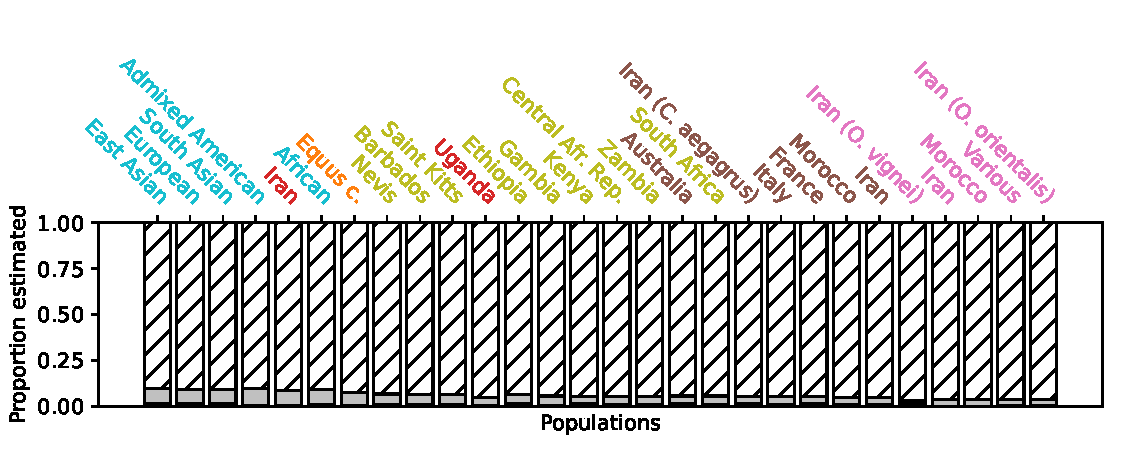
\includegraphics[width=\linewidth, page=1]{artworks/Theta.neg.stacked.pdf}
    \end{minipage}
    \begin{minipage}{0.09\linewidth}
        
\includegraphics[width=\linewidth, page=1]{artworks/legend.polycat}
    \end{minipage}

    \newpage

    \captionof{figure}{Estimation of selection at the population scale for $\SphyNeu$ mutations}
    \begin{minipage}{0.9\linewidth}
        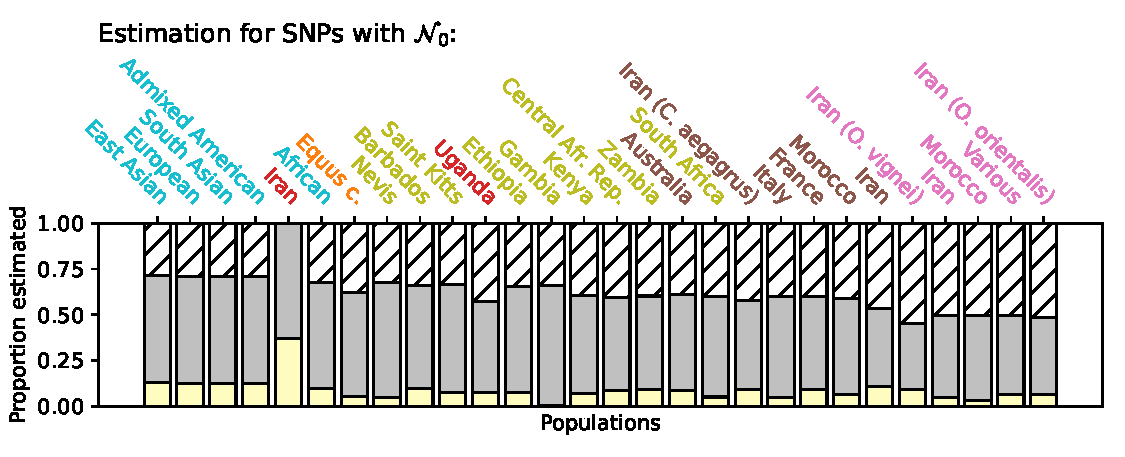
\includegraphics[width=\linewidth, page=1]{artworks/Theta.weak.stacked.pdf}
    \end{minipage}
    \begin{minipage}{0.09\linewidth}
        
\includegraphics[width=\linewidth, page=1]{artworks/legend.polycat}
    \end{minipage}

    \captionof{figure}{Estimation of selection at the population scale for $\SphyBen$ mutations}
    \begin{minipage}{0.9\linewidth}
        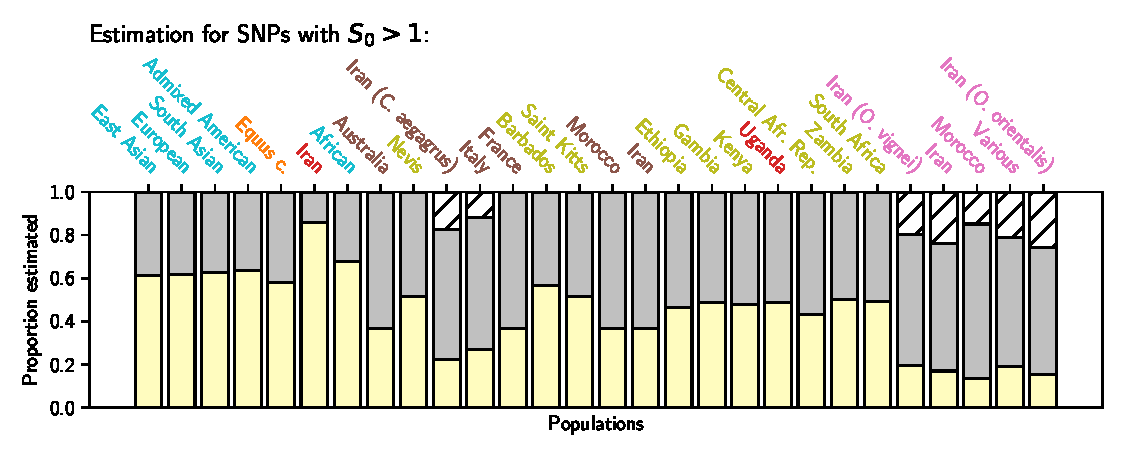
\includegraphics[width=\linewidth, page=1]{artworks/Theta.pos.stacked.pdf}
    \end{minipage}
    \begin{minipage}{0.09\linewidth}
        
\includegraphics[width=\linewidth, page=1]{artworks/legend.polycat}
    \end{minipage}

    \newpage

    \section{Including divergence data for the estimation of $\Spop$}

    \subsection{Including divergence in polyDFE}
    Divergence data (number of substitutions per site) can also be included into polyDFE to estimate the DFE.
    For the class of a given class of selection coefficient ($\Sphyclass \in \{\SphyDel, \SphyNeu, \SphyBen \}$), the number of substitutions has already been computed and is given by $D\left( \Sphyclass \right)$ (see eq.~6), and the number of sites is given by $L \left( \Sphyclass \right)$ (see eq.~4).
    Otherwise, the procedure is the same as described section \textit{Scaled selection coefficients ($\Spop$) in a population-based method}.

    \subsection{Probabilities of beneficial back-mutations}
    \begin{center}
        \captionof{table}{Probability of beneficial back-mutations among all beneficial ones - including divergence.}
        \scriptsize
        \begin{longtable*}{|l|l|r|r|r|r|r|r|}
            \toprule
            Population & Species & $\Ne$ & $\proba[\SphyBen]$ & $\proba [ \SpopBen ]$ & $\frac{\proba[\SphyBen]}{\proba[ \SpopBen ]}$ & $\proba [ \SpopBen \given \SphyBen]$ & $\proba[\SphyBen\given \SpopBen ]$ \\
            \midrule
            \endhead
            \midrule
            \multicolumn{8}{r}{{Continued on next page}} \\
            \midrule
            \endfoot

            \bottomrule
            \endlastfoot
            \rowcolor{LIGHTGREY} Equus c. & Equus caballus & $7.5\times 10^{4}$ & $ 0.012$ & $ 0.057$ & $ 0.213$ & $ 0.498$ & $ 0.106$ \\
            Iran & Bos taurus & $5.6\times 10^{4}$ & $ 0.011$ & $ 0.006$ & $ 1.860$ & $ 0.368$ & $ 0.684$ \\
            Uganda & Bos taurus & $1.3\times 10^{5}$ & $ 0.011$ & $ 0.012$ & $ 0.900$ & $ 0.307$ & $ 0.276$ \\
            \rowcolor{LIGHTGREY} Australia & Capra hircus & $1.7\times 10^{5}$ & $ 0.011$ & $ 0.007$ & $ 1.651$ & $ 0.178$ & $ 0.294$ \\
            \rowcolor{LIGHTGREY} France & Capra hircus & $1.9\times 10^{5}$ & $ 0.011$ & $ 0.007$ & $ 1.614$ & $ 0.183$ & $ 0.295$ \\
            \rowcolor{LIGHTGREY} Iran (C. aegagrus) & Capra hircus & $1.9\times 10^{5}$ & $ 0.011$ & $ 0.012$ & $ 0.923$ & $ 0.177$ & $ 0.163$ \\
            \rowcolor{LIGHTGREY} Iran & Capra hircus & $2.3\times 10^{5}$ & $ 0.011$ & $ 0.008$ & $ 1.483$ & $ 0.184$ & $ 0.273$ \\
            \rowcolor{LIGHTGREY} Italy & Capra hircus & $1.9\times 10^{5}$ & $ 0.011$ & $ 0.007$ & $ 1.686$ & $ 0.178$ & $ 0.299$ \\
            \rowcolor{LIGHTGREY} Morocco & Capra hircus & $2.2\times 10^{5}$ & $ 0.011$ & $ 0.006$ & $ 1.892$ & $ 0.184$ & $ 0.349$ \\
            Iran & Ovis aries & $3.8\times 10^{5}$ & $ 0.012$ & $ 0.010$ & $ 1.132$ & $ 0.189$ & $ 0.214$ \\
            Iran (O. orientalis) & Ovis aries & $4.5\times 10^{5}$ & $ 0.011$ & $ 0.011$ & $ 1.012$ & $ 0.213$ & $ 0.216$ \\
            Iran (O. vignei) & Ovis aries & $3.7\times 10^{5}$ & $ 0.012$ & $ 0.021$ & $ 0.561$ & $ 0.186$ & $ 0.105$ \\
            Various & Ovis aries & $4.1\times 10^{5}$ & $ 0.011$ & $ 0.011$ & $ 1.069$ & $ 0.215$ & $ 0.229$ \\
            Morocco & Ovis aries & $ 4\times 10^{5}$ & $ 0.012$ & $ 0.012$ & $ 0.973$ & $ 0.217$ & $ 0.211$ \\
            \rowcolor{LIGHTGREY} Barbados & Chlorocebus sabaeus & $1.1\times 10^{5}$ & $ 0.009$ & $ 0.004$ & $ 2.120$ & $ 0.341$ & $ 0.723$ \\
            \rowcolor{LIGHTGREY} Central Afr. Rep. & Chlorocebus sabaeus & $1.7\times 10^{5}$ & $ 0.009$ & $ 0.013$ & $ 0.720$ & $ 0.368$ & $ 0.265$ \\
            \rowcolor{LIGHTGREY} Ethiopia & Chlorocebus sabaeus & $1.4\times 10^{5}$ & $ 0.009$ & $ 0.007$ & $ 1.352$ & $ 0.368$ & $ 0.498$ \\
            \rowcolor{LIGHTGREY} Gambia & Chlorocebus sabaeus & $1.4\times 10^{5}$ & $ 0.009$ & $ 0.010$ & $ 0.956$ & $ 0.368$ & $ 0.352$ \\
            \rowcolor{LIGHTGREY} Kenya & Chlorocebus sabaeus & $1.5\times 10^{5}$ & $ 0.009$ & $ 0.013$ & $ 0.727$ & $ 0.368$ & $ 0.268$ \\
            \rowcolor{LIGHTGREY} Nevis & Chlorocebus sabaeus & $ 1\times 10^{5}$ & $ 0.009$ & $ 0.004$ & $ 2.133$ & $ 0.368$ & $ 0.784$ \\
            \rowcolor{LIGHTGREY} South Africa & Chlorocebus sabaeus & $1.8\times 10^{5}$ & $ 0.009$ & $ 0.011$ & $ 0.874$ & $ 0.368$ & $ 0.322$ \\
            \rowcolor{LIGHTGREY} Saint Kitts & Chlorocebus sabaeus & $1.2\times 10^{5}$ & $ 0.009$ & $ 0.005$ & $ 1.905$ & $ 0.368$ & $ 0.701$ \\
            \rowcolor{LIGHTGREY} Zambia & Chlorocebus sabaeus & $1.7\times 10^{5}$ & $ 0.009$ & $ 0.014$ & $ 0.698$ & $ 0.368$ & $ 0.257$ \\
            African & Homo sapiens & $5.6\times 10^{4}$ & $ 0.010$ & $ 0.013$ & $ 0.726$ & $ 0.437$ & $ 0.317$ \\
            Admixed American & Homo sapiens & $4.5\times 10^{4}$ & $ 0.010$ & $ 0.011$ & $ 0.886$ & $ 0.429$ & $ 0.380$ \\
            East Asian & Homo sapiens & $ 4\times 10^{4}$ & $ 0.010$ & $ 0.008$ & $ 1.213$ & $ 0.426$ & $ 0.517$ \\
            European & Homo sapiens & $4.1\times 10^{4}$ & $ 0.010$ & $ 0.009$ & $ 1.104$ & $ 0.422$ & $ 0.466$ \\
            South Asian & Homo sapiens & $4.4\times 10^{4}$ & $ 0.010$ & $ 0.009$ & $ 1.016$ & $ 0.426$ & $ 0.433$ \\
        \end{longtable*}
    \end{center}
    \begin{itemize}
        \item $\Ne$ is the estimated effective population size.
        \item $\proba [ \SphyBen ]$ (eq.~5) is the probability for a new mutation a beneficial back-mutation.
        These mutations have a selection coefficient predicted at the phylogenetic-scale larger than 1, thus toward a more fit amino-acid.
        \item $\proba [ \SpopBen ]$ (eq.~15) is the probability for a mutation to be beneficial.
        These mutations have a selection coefficient at the population-scale larger than 1.
        \item $\proba [ \SpopBen \given \SphyBen]$ (eq.~12) is the probability for a mutation to be beneficial at the population scale, given it is predicted to be a beneficial back-mutation at the phylogenetic scale (the \textit{precision}).
        \item $\proba [ \SphyBen \given \SpopBen]$ (eq.~14) is the probability for a mutation to a beneficial back-mutations, given it is beneficial (the \textit{recall}).
        This probability is obtained using Bayes' formula.
    \end{itemize}
    \newpage

    \subsection{Precision and recall}
    \captionof{table}{Precision and recall - including divergence}
    \begin{center}
        \begin{adjustbox}{width=\textwidth}
            \begin{tabular}{||l|l|r||r|r||r|r||r|r||}
                \toprule
                \multicolumn{3}{||c||}{} &
                \multicolumn{2}{c||}{\shortstack{\textbf{Deleterious mutations} \\ $\bm{\SpopDel \coloneqq \Spop<-1}$ \\ $\bm{\SphyDel \coloneqq \Sphy<-1}$}} &
                \multicolumn{2}{c||}{\shortstack{\textbf{Nearly-neutral mutations} \\ $\bm{\SpopNeu \coloneqq -1<\Spop<1}$ \\ $\bm{\SphyNeu \coloneqq -1<\Sphy<1}$}} &
                \multicolumn{2}{c||}{\shortstack{\textbf{Beneficial mutations} \\ $\bm{\SpopBen \coloneqq \Spop>1}$ \\ $\bm{\SphyBen \coloneqq \Sphy>1}$}}
                \\ \hline
                \textbf{Population} &
                \textbf{Species} &
                $\bm{\Ne}$ &
                \makecell{\textbf{Precision} \\ $\bm{\proba [\SpopDel \given \SphyDel]}$} &
                \makecell{\textbf{Recall} \\ $\bm{\proba [\SphyDel \given \SpopDel]}$}           &
                \makecell{\textbf{Precision}      \\ $\bm{\proba [\SpopNeu \given \SphyNeu]}$}                                    &
                \makecell{\textbf{Recall}          \\ $\bm{\proba [\SphyNeu \given \SpopNeu]}$}                                  &
                \makecell{\textbf{Precision}          \\ $\bm{\proba [\SpopBen \given \SphyBen]}$}          &
                \makecell{\textbf{Recall}        \\ $\bm{\proba [\SphyBen \given \SpopBen]}$}
                \\   \midrule
                \rowcolor{LIGHTGREY} Equus c. & Equus caballus & $7.5\times 10^{4}$ & $ 0.937$ & $ 0.955$ & $ 0.111$ & $ 0.192$ & $ 0.498$ & $ 0.106$ \\
                Iran & Bos taurus & $5.6\times 10^{4}$ & $ 0.935$ & $ 0.970$ & $ 0.565$ & $ 0.356$ & $ 0.368$ & $ 0.684$ \\
                Uganda & Bos taurus & $1.3\times 10^{5}$ & $ 0.951$ & $ 0.967$ & $ 0.516$ & $ 0.422$ & $ 0.307$ & $ 0.276$ \\
                \rowcolor{LIGHTGREY} Australia & Capra hircus & $1.7\times 10^{5}$ & $ 0.952$ & $ 0.970$ & $ 0.598$ & $ 0.452$ & $ 0.178$ & $ 0.294$ \\
                \rowcolor{LIGHTGREY} France & Capra hircus & $1.9\times 10^{5}$ & $ 0.951$ & $ 0.969$ & $ 0.574$ & $ 0.433$ & $ 0.183$ & $ 0.295$ \\
                \rowcolor{LIGHTGREY} Iran (C. aegagrus) & Capra hircus & $1.9\times 10^{5}$ & $ 0.957$ & $ 0.966$ & $ 0.515$ & $ 0.460$ & $ 0.177$ & $ 0.163$ \\
                \rowcolor{LIGHTGREY} Iran & Capra hircus & $2.3\times 10^{5}$ & $ 0.951$ & $ 0.967$ & $ 0.542$ & $ 0.422$ & $ 0.184$ & $ 0.273$ \\
                \rowcolor{LIGHTGREY} Italy & Capra hircus & $1.9\times 10^{5}$ & $ 0.951$ & $ 0.969$ & $ 0.582$ & $ 0.436$ & $ 0.178$ & $ 0.299$ \\
                \rowcolor{LIGHTGREY} Morocco & Capra hircus & $2.2\times 10^{5}$ & $ 0.949$ & $ 0.968$ & $ 0.556$ & $ 0.412$ & $ 0.184$ & $ 0.349$ \\
                Iran & Ovis aries & $3.8\times 10^{5}$ & $ 0.963$ & $ 0.962$ & $ 0.421$ & $ 0.424$ & $ 0.189$ & $ 0.214$ \\
                Iran (O. orientalis) & Ovis aries & $4.5\times 10^{5}$ & $ 0.968$ & $ 0.961$ & $ 0.413$ & $ 0.460$ & $ 0.213$ & $ 0.216$ \\
                Iran (O. vignei) & Ovis aries & $3.7\times 10^{5}$ & $ 0.972$ & $ 0.959$ & $ 0.360$ & $ 0.528$ & $ 0.186$ & $ 0.105$ \\
                Various & Ovis aries & $4.1\times 10^{5}$ & $ 0.966$ & $ 0.961$ & $ 0.430$ & $ 0.454$ & $ 0.215$ & $ 0.229$ \\
                Morocco & Ovis aries & $ 4\times 10^{5}$ & $ 0.966$ & $ 0.958$ & $ 0.372$ & $ 0.416$ & $ 0.217$ & $ 0.211$ \\
                \rowcolor{LIGHTGREY} Barbados & Chlorocebus sabaeus & $1.1\times 10^{5}$ & $ 0.940$ & $ 0.976$ & $ 0.654$ & $ 0.409$ & $ 0.341$ & $ 0.723$ \\
                \rowcolor{LIGHTGREY} Central Afr. Rep. & Chlorocebus sabaeus & $1.7\times 10^{5}$ & $ 0.950$ & $ 0.971$ & $ 0.526$ & $ 0.421$ & $ 0.368$ & $ 0.265$ \\
                \rowcolor{LIGHTGREY} Ethiopia & Chlorocebus sabaeus & $1.4\times 10^{5}$ & $ 0.942$ & $ 0.974$ & $ 0.609$ & $ 0.402$ & $ 0.368$ & $ 0.498$ \\
                \rowcolor{LIGHTGREY} Gambia & Chlorocebus sabaeus & $1.4\times 10^{5}$ & $ 0.950$ & $ 0.974$ & $ 0.611$ & $ 0.452$ & $ 0.368$ & $ 0.352$ \\
                \rowcolor{LIGHTGREY} Kenya & Chlorocebus sabaeus & $1.5\times 10^{5}$ & $ 0.950$ & $ 0.972$ & $ 0.545$ & $ 0.434$ & $ 0.368$ & $ 0.268$ \\
                \rowcolor{LIGHTGREY} Nevis & Chlorocebus sabaeus & $ 1\times 10^{5}$ & $ 0.940$ & $ 0.977$ & $ 0.668$ & $ 0.412$ & $ 0.368$ & $ 0.784$ \\
                \rowcolor{LIGHTGREY} South Africa & Chlorocebus sabaeus & $1.8\times 10^{5}$ & $ 0.947$ & $ 0.972$ & $ 0.550$ & $ 0.411$ & $ 0.368$ & $ 0.322$ \\
                \rowcolor{LIGHTGREY} Saint Kitts & Chlorocebus sabaeus & $1.2\times 10^{5}$ & $ 0.940$ & $ 0.976$ & $ 0.646$ & $ 0.407$ & $ 0.368$ & $ 0.701$ \\
                \rowcolor{LIGHTGREY} Zambia & Chlorocebus sabaeus & $1.7\times 10^{5}$ & $ 0.950$ & $ 0.971$ & $ 0.527$ & $ 0.426$ & $ 0.368$ & $ 0.257$ \\
                African & Homo sapiens & $5.6\times 10^{4}$ & $ 0.911$ & $ 0.980$ & $ 0.666$ & $ 0.341$ & $ 0.437$ & $ 0.317$ \\
                Admixed American & Homo sapiens & $4.5\times 10^{4}$ & $ 0.902$ & $ 0.976$ & $ 0.580$ & $ 0.284$ & $ 0.429$ & $ 0.380$ \\
                East Asian & Homo sapiens & $ 4\times 10^{4}$ & $ 0.904$ & $ 0.984$ & $ 0.744$ & $ 0.341$ & $ 0.426$ & $ 0.517$ \\
                European & Homo sapiens & $4.1\times 10^{4}$ & $ 0.906$ & $ 0.984$ & $ 0.737$ & $ 0.344$ & $ 0.422$ & $ 0.466$ \\
                South Asian & Homo sapiens & $4.4\times 10^{4}$ & $ 0.907$ & $ 0.984$ & $ 0.737$ & $ 0.349$ & $ 0.426$ & $ 0.433$ \\
                \bottomrule
            \end{tabular}
        \end{adjustbox}
    \end{center}
    \begin{itemize}
        \item $\Ne$ is the estimated effective population size.
        \item \textit{Precision} is the estimation of the selection coefficient at population scale ($\Spop$) given that $\Sphy$ is known.
        \item  \textit{Recall} is the estimation of $\Sphy$ given selection coefficient at the population scale ($\Spop$) is known.
        \item \textit{Recall} for beneficial mutations ($\proba [\SphyBen \given \SpopBen]$) is thus the proportion of beneficial back-mutations among all beneficial mutations.
    \end{itemize}

    Altogether, comparing this table to tables 1 and S3, we acknowledge that the exact proportion of beneficial back-mutations among all beneficial ones is different whether we included or not substitutions in the terminal lineage for the estimation of $\Spop$.
    However, we can still see that beneficial back-mutations are positively selected compared to neutral and deleterious ones, and this result is not sensitive to inclusion of substitutions in the terminal lineage.
    \newpage

    \subsection{Excluding genes under adaptation}

    \begin{center}
        \captionof{table}{$\proba[\SphyBen\given \SpopBen ]$ for each population when excluding or not genes under adaptation - including divergence.}
        \begin{tabular}{|l|l|r|r|}
            \toprule
            Population & Species & Control & Case \\
            \midrule
            \rowcolor{LIGHTGREY} Equus c. & Equus caballus & $ 0.106$ & $ 0.106$ \\
            Iran & Bos taurus & $ 0.684$ & $ 0.755$ \\
            Uganda & Bos taurus & $ 0.276$ & $ 0.310$ \\
            \rowcolor{LIGHTGREY} Australia & Capra hircus & $ 0.294$ & $ 0.319$ \\
            \rowcolor{LIGHTGREY} France & Capra hircus & $ 0.295$ & $ 0.325$ \\
            \rowcolor{LIGHTGREY} Iran (C. aegagrus) & Capra hircus & $ 0.163$ & $ 0.174$ \\
            \rowcolor{LIGHTGREY} Iran & Capra hircus & $ 0.273$ & $ 0.299$ \\
            \rowcolor{LIGHTGREY} Italy & Capra hircus & $ 0.299$ & $ 0.321$ \\
            \rowcolor{LIGHTGREY} Morocco & Capra hircus & $ 0.349$ & $ 0.419$ \\
            Iran & Ovis aries & $ 0.214$ & $ 0.241$ \\
            Iran (O. orientalis) & Ovis aries & $ 0.216$ & $ 0.213$ \\
            Iran (O. vignei) & Ovis aries & $ 0.105$ & $ 0.089$ \\
            Various & Ovis aries & $ 0.229$ & $ 0.196$ \\
            Morocco & Ovis aries & $ 0.211$ & $ 0.206$ \\
            \rowcolor{LIGHTGREY} Barbados & Chlorocebus sabaeus & $ 0.723$ & $ 0.833$ \\
            \rowcolor{LIGHTGREY} Central Afr. Rep. & Chlorocebus sabaeus & $ 0.265$ & $ 0.285$ \\
            \rowcolor{LIGHTGREY} Ethiopia & Chlorocebus sabaeus & $ 0.498$ & $ 0.547$ \\
            \rowcolor{LIGHTGREY} Gambia & Chlorocebus sabaeus & $ 0.352$ & $ 0.571$ \\
            \rowcolor{LIGHTGREY} Kenya & Chlorocebus sabaeus & $ 0.268$ & $ 0.265$ \\
            \rowcolor{LIGHTGREY} Nevis & Chlorocebus sabaeus & $ 0.784$ & $ 0.892$ \\
            \rowcolor{LIGHTGREY} South Africa & Chlorocebus sabaeus & $ 0.322$ & $ 0.307$ \\
            \rowcolor{LIGHTGREY} Saint Kitts & Chlorocebus sabaeus & $ 0.701$ & $ 0.825$ \\
            \rowcolor{LIGHTGREY} Zambia & Chlorocebus sabaeus & $ 0.257$ & $ 0.271$ \\
            African & Homo sapiens & $ 0.317$ & $ 0.278$ \\
            Admixed American & Homo sapiens & $ 0.380$ & $ 0.363$ \\
            East Asian & Homo sapiens & $ 0.517$ & $ 0.499$ \\
            European & Homo sapiens & $ 0.466$ & $ 0.456$ \\
            South Asian & Homo sapiens & $ 0.433$ & $ 0.304$ \\
            \bottomrule
        \end{tabular}
    \end{center}
    Genes under adaptation retrieved from~\cite{latrille_genes_2023}.
    Comparison of $\proba[\SphyBen\given \SpopBen ]$ while including divergence for the whole genome (control) and when excluding genes under adaptation (case).
    The non-parametric Wilcoxon signed-rank test tests the null hypothesis that the distribution of the differences (case versus control) is symmetric about zero.
    Applied to the paired samples (case and control), Wilcoxon signed-rank test results in $s=120$ with $\pvalue=0.027$ for one-sided test (case higher than control).
    The proportion of beneficial back-mutations ($\proba[\SphyBen\given \SpopBen ]$) is higher when excluding genes under adaptation, consistent with our expectation that genes with uniformly conserved functions should fit better the back-mutation equilibrium model.

    \newpage

    \section{Discrete distribution of $\Spop$ at the population scale}

    \subsection{polyDFE model D (discrete distribution)}
    Additionally to including divergence, with also tested our prediction with polyDFE model D instead of model C.
    In polyDFE model D, the DFE of non-synonymous mutations is given as a discrete DFE of $K$ categories (instead of a continuous distribution in model C), where the selection coefficients of each category $i$ ($1 \leq i \leq K$) are fixed parameters $\Spop_i$, and each value $\Spop_i$ has a probability $p_i$ (estimated), with $\sum_{i=1}^{K} p_i =1$.
    We used $K=6$ with $\Spop_1 = -500$, $\Spop_2 = -4$, $\Spop_3 =-1$, $\Spop_4 = 0$, $\Spop_5 = 1$, $\Spop_6 = 4$.\\
    For each class of selection $\Sphyclass$, the parameters $p_i$ ($i \in \{ 1 \leq i \leq 6 \}$) were used to compute $\proba [ \SpopDel \given  \Sphyclass] $, $\proba [ \SpopNeu \given \Sphyclass]$, and $\proba [ \SpopBen \given \Sphyclass]$ as:
    \begin{align}
        \proba [ \SpopDel \given  \Sphyclass] &= \proba [ \Spop < -1 \given \Sphyclass ] = p_1 + p_2 \label{eq:polyProbaDel-mD} \\
        \proba [ \SpopNeu \given \Sphyclass] &= \proba [ -1 < \Spop < 1 \given \Sphyclass ] = p_3 + p_4 + p_5,  \\
        \proba [ \SpopBen \given \Sphyclass] &= \proba [  \Spop > 1 \given \Sphyclass ] = p_6.  \label{eq:polyProbaAdv-mD}
    \end{align}

    \subsection{Probabilities of beneficial back-mutations}
    \begin{center}
        \captionof{table}{Probability of beneficial back-mutations among all beneficial ones - model D.}
        \scriptsize
        \begin{longtable*}{|l|l|r|r|r|r|r|r|}
            \toprule
            Population & Species & $\Ne$ & $\proba[\SphyBen]$ & $\proba [ \SpopBen ]$ & $\frac{\proba[\SphyBen]}{\proba[ \SpopBen ]}$ & $\proba [ \SpopBen \given \SphyBen]$ & $\proba[\SphyBen\given \SpopBen ]$ \\
            \midrule
            \endhead
            \midrule
            \multicolumn{8}{r}{{Continued on next page}} \\
            \midrule
            \endfoot

            \bottomrule
            \endlastfoot
            \rowcolor{LIGHTGREY} Equus c. & Equus caballus & $7.5\times 10^{4}$ & $ 0.012$ & $ 0.006$ & $ 2.050$ & $ 0.163$ & $ 0.334$ \\
            Iran & Bos taurus & $5.6\times 10^{4}$ & $ 0.011$ & $ 0.005$ & $ 2.125$ & $ 0.133$ & $ 0.283$ \\
            Uganda & Bos taurus & $1.3\times 10^{5}$ & $ 0.011$ & $ 0.010$ & $ 1.139$ & $ 0.140$ & $ 0.159$ \\
            \rowcolor{LIGHTGREY} Australia & Capra hircus & $1.7\times 10^{5}$ & $ 0.011$ & $ 0.002$ & $ 5.637$ & $ 0.151$ & $ 0.850$ \\
            \rowcolor{LIGHTGREY} France & Capra hircus & $1.9\times 10^{5}$ & $ 0.011$ & $ 0.002$ & $ 6.117$ & $ 0.154$ & $ 0.940$ \\
            \rowcolor{LIGHTGREY} Iran (C. aegagrus) & Capra hircus & $1.9\times 10^{5}$ & $ 0.011$ & $ 0.002$ & $ 5.842$ & $ 0.156$ & $ 0.911$ \\
            \rowcolor{LIGHTGREY} Iran & Capra hircus & $2.3\times 10^{5}$ & $ 0.011$ & $ 0.002$ & $ 6.400$ & $ 0.147$ & $ 0.943$ \\
            \rowcolor{LIGHTGREY} Italy & Capra hircus & $1.9\times 10^{5}$ & $ 0.011$ & $ 0.002$ & $ 5.793$ & $ 0.155$ & $ 0.895$ \\
            \rowcolor{LIGHTGREY} Morocco & Capra hircus & $2.2\times 10^{5}$ & $ 0.011$ & $ 0.003$ & $ 4.192$ & $ 0.150$ & $ 0.627$ \\
            Iran & Ovis aries & $3.8\times 10^{5}$ & $ 0.012$ & $ 0.020$ & $ 0.584$ & $ 0.154$ & $ 0.090$ \\
            Iran (O. orientalis) & Ovis aries & $4.5\times 10^{5}$ & $ 0.011$ & $ 0.021$ & $ 0.535$ & $ 0.148$ & $ 0.079$ \\
            Iran (O. vignei) & Ovis aries & $3.7\times 10^{5}$ & $ 0.012$ & $ 0.020$ & $ 0.568$ & $ 0.151$ & $ 0.086$ \\
            Various & Ovis aries & $4.1\times 10^{5}$ & $ 0.011$ & $ 0.021$ & $ 0.553$ & $ 0.152$ & $ 0.084$ \\
            Morocco & Ovis aries & $ 4\times 10^{5}$ & $ 0.012$ & $ 0.022$ & $ 0.529$ & $ 0.153$ & $ 0.081$ \\
            \rowcolor{LIGHTGREY} Barbados & Chlorocebus sabaeus & $1.1\times 10^{5}$ & $ 0.009$ & $ 0.002$ & $ 5.152$ & $ 0.170$ & $ 0.877$ \\
            \rowcolor{LIGHTGREY} Central Afr. Rep. & Chlorocebus sabaeus & $1.7\times 10^{5}$ & $ 0.009$ & $ 0.007$ & $ 1.266$ & $ 0.157$ & $ 0.199$ \\
            \rowcolor{LIGHTGREY} Ethiopia & Chlorocebus sabaeus & $1.4\times 10^{5}$ & $ 0.009$ & $ 0.002$ & $ 3.979$ & $ 0.161$ & $ 0.640$ \\
            \rowcolor{LIGHTGREY} Gambia & Chlorocebus sabaeus & $1.4\times 10^{5}$ & $ 0.009$ & $ 0.008$ & $ 1.201$ & $ 0.159$ & $ 0.191$ \\
            \rowcolor{LIGHTGREY} Kenya & Chlorocebus sabaeus & $1.5\times 10^{5}$ & $ 0.009$ & $ 0.003$ & $ 2.801$ & $ 0.165$ & $ 0.461$ \\
            \rowcolor{LIGHTGREY} Nevis & Chlorocebus sabaeus & $ 1\times 10^{5}$ & $ 0.009$ & $ 0.002$ & $ 5.361$ & $ 0.169$ & $ 0.908$ \\
            \rowcolor{LIGHTGREY} South Africa & Chlorocebus sabaeus & $1.8\times 10^{5}$ & $ 0.009$ & $ 0.005$ & $ 1.912$ & $ 0.154$ & $ 0.294$ \\
            \rowcolor{LIGHTGREY} Saint Kitts & Chlorocebus sabaeus & $1.2\times 10^{5}$ & $ 0.009$ & $ 0.002$ & $ 4.561$ & $ 0.165$ & $ 0.753$ \\
            \rowcolor{LIGHTGREY} Zambia & Chlorocebus sabaeus & $1.7\times 10^{5}$ & $ 0.009$ & $ 0.004$ & $ 2.661$ & $ 0.153$ & $ 0.406$ \\
            African & Homo sapiens & $5.6\times 10^{4}$ & $ 0.010$ & $ 0.010$ & $ 0.997$ & $ 0.154$ & $ 0.154$ \\
            Admixed American & Homo sapiens & $4.5\times 10^{4}$ & $ 0.010$ & $ 0.008$ & $ 1.206$ & $ 0.158$ & $ 0.190$ \\
            East Asian & Homo sapiens & $ 4\times 10^{4}$ & $ 0.010$ & $ 0.007$ & $ 1.455$ & $ 0.163$ & $ 0.237$ \\
            European & Homo sapiens & $4.2\times 10^{4}$ & $ 0.010$ & $ 0.007$ & $ 1.316$ & $ 0.167$ & $ 0.219$ \\
            South Asian & Homo sapiens & $4.4\times 10^{4}$ & $ 0.010$ & $ 0.007$ & $ 1.340$ & $ 0.164$ & $ 0.219$ \\
        \end{longtable*}
    \end{center}
    \begin{itemize}
        \item $\Ne$ is the estimated effective population size.
        \item $\proba [ \SphyBen ]$ (eq.~5) is the probability for a new mutation a beneficial back-mutation.
        These mutations have a selection coefficient predicted at the phylogenetic-scale larger than 1, thus toward a more fit amino-acid.
        \item $\proba [ \SpopBen ]$ (eq.~15) is the probability for a mutation to be beneficial.
        These mutations have a selection coefficient at the population-scale larger than 1.
        \item $\proba [ \SpopBen \given \SphyBen]$ (eq.~12) is the probability for a mutation to be beneficial at the population scale, given it is predicted to be a beneficial back-mutation at the phylogenetic scale (the \textit{precision}).
        \item $\proba [ \SphyBen \given \SpopBen]$ (eq.~14) is the probability for a mutation to a beneficial back-mutations, given it is beneficial (the \textit{recall}).
        This probability is obtained using Bayes' formula.
    \end{itemize}
    \newpage

    \subsection{Precision and recall}
    \captionof{table}{Precision and recall - model D}
    \begin{center}
        \begin{adjustbox}{width=\textwidth}
            \begin{tabular}{||l|l|r||r|r||r|r||r|r||}
                \toprule
                \multicolumn{3}{||c||}{} &
                \multicolumn{2}{c||}{\shortstack{\textbf{Deleterious mutations} \\ $\bm{\SpopDel \coloneqq \Spop<-1}$ \\ $\bm{\SphyDel \coloneqq \Sphy<-1}$}} &
                \multicolumn{2}{c||}{\shortstack{\textbf{Nearly-neutral mutations} \\ $\bm{\SpopNeu \coloneqq -1<\Spop<1}$ \\ $\bm{\SphyNeu \coloneqq -1<\Sphy<1}$}} &
                \multicolumn{2}{c||}{\shortstack{\textbf{Beneficial mutations} \\ $\bm{\SpopBen \coloneqq \Spop>1}$ \\ $\bm{\SphyBen \coloneqq \Sphy>1}$}}
                \\ \hline
                \textbf{Population} &
                \textbf{Species} &
                $\bm{\Ne}$ &
                \makecell{\textbf{Precision} \\ $\bm{\proba [\SpopDel \given \SphyDel]}$} &
                \makecell{\textbf{Recall} \\ $\bm{\proba [\SphyDel \given \SpopDel]}$}           &
                \makecell{\textbf{Precision}      \\ $\bm{\proba [\SpopNeu \given \SphyNeu]}$}                                    &
                \makecell{\textbf{Recall}          \\ $\bm{\proba [\SphyNeu \given \SpopNeu]}$}                                  &
                \makecell{\textbf{Precision}          \\ $\bm{\proba [\SpopBen \given \SphyBen]}$}          &
                \makecell{\textbf{Recall}        \\ $\bm{\proba [\SphyBen \given \SpopBen]}$}
                \\   \midrule
                \rowcolor{LIGHTGREY} Equus c. & Equus caballus & $7.5\times 10^{4}$ & $ 0.911$ & $ 0.974$ & $ 0.645$ & $ 0.319$ & $ 0.163$ & $ 0.334$ \\
                Iran & Bos taurus & $5.6\times 10^{4}$ & $ 0.895$ & $ 0.973$ & $ 0.639$ & $ 0.288$ & $ 0.133$ & $ 0.283$ \\
                Uganda & Bos taurus & $1.3\times 10^{5}$ & $ 0.951$ & $ 0.974$ & $ 0.664$ & $ 0.492$ & $ 0.140$ & $ 0.159$ \\
                \rowcolor{LIGHTGREY} Australia & Capra hircus & $1.7\times 10^{5}$ & $ 0.912$ & $ 0.984$ & $ 0.834$ & $ 0.386$ & $ 0.151$ & $ 0.850$ \\
                \rowcolor{LIGHTGREY} France & Capra hircus & $1.9\times 10^{5}$ & $ 0.912$ & $ 0.983$ & $ 0.819$ & $ 0.381$ & $ 0.154$ & $ 0.940$ \\
                \rowcolor{LIGHTGREY} Iran (C. aegagrus) & Capra hircus & $1.9\times 10^{5}$ & $ 0.928$ & $ 0.980$ & $ 0.767$ & $ 0.408$ & $ 0.156$ & $ 0.911$ \\
                \rowcolor{LIGHTGREY} Iran & Capra hircus & $2.3\times 10^{5}$ & $ 0.955$ & $ 0.969$ & $ 0.616$ & $ 0.459$ & $ 0.147$ & $ 0.943$ \\
                \rowcolor{LIGHTGREY} Italy & Capra hircus & $1.9\times 10^{5}$ & $ 0.911$ & $ 0.983$ & $ 0.822$ & $ 0.379$ & $ 0.155$ & $ 0.895$ \\
                \rowcolor{LIGHTGREY} Morocco & Capra hircus & $2.2\times 10^{5}$ & $ 0.950$ & $ 0.976$ & $ 0.706$ & $ 0.468$ & $ 0.150$ & $ 0.627$ \\
                Iran & Ovis aries & $3.8\times 10^{5}$ & $ 0.983$ & $ 0.958$ & $ 0.421$ & $ 0.796$ & $ 0.154$ & $ 0.090$ \\
                Iran (O. orientalis) & Ovis aries & $4.5\times 10^{5}$ & $ 0.982$ & $ 0.961$ & $ 0.448$ & $ 0.806$ & $ 0.148$ & $ 0.079$ \\
                Iran (O. vignei) & Ovis aries & $3.7\times 10^{5}$ & $ 0.974$ & $ 0.963$ & $ 0.480$ & $ 0.685$ & $ 0.151$ & $ 0.086$ \\
                Various & Ovis aries & $4.1\times 10^{5}$ & $ 0.982$ & $ 0.964$ & $ 0.500$ & $ 0.822$ & $ 0.152$ & $ 0.084$ \\
                Morocco & Ovis aries & $ 4\times 10^{5}$ & $ 0.983$ & $ 0.958$ & $ 0.387$ & $ 0.782$ & $ 0.153$ & $ 0.081$ \\
                \rowcolor{LIGHTGREY} Barbados & Chlorocebus sabaeus & $1.1\times 10^{5}$ & $ 0.895$ & $ 0.987$ & $ 0.860$ & $ 0.351$ & $ 0.170$ & $ 0.877$ \\
                \rowcolor{LIGHTGREY} Central Afr. Rep. & Chlorocebus sabaeus & $1.7\times 10^{5}$ & $ 0.925$ & $ 0.974$ & $ 0.653$ & $ 0.373$ & $ 0.157$ & $ 0.199$ \\
                \rowcolor{LIGHTGREY} Ethiopia & Chlorocebus sabaeus & $1.4\times 10^{5}$ & $ 0.892$ & $ 0.980$ & $ 0.763$ & $ 0.320$ & $ 0.161$ & $ 0.640$ \\
                \rowcolor{LIGHTGREY} Gambia & Chlorocebus sabaeus & $1.4\times 10^{5}$ & $ 0.939$ & $ 0.982$ & $ 0.770$ & $ 0.469$ & $ 0.159$ & $ 0.191$ \\
                \rowcolor{LIGHTGREY} Kenya & Chlorocebus sabaeus & $1.5\times 10^{5}$ & $ 0.916$ & $ 0.976$ & $ 0.680$ & $ 0.345$ & $ 0.165$ & $ 0.461$ \\
                \rowcolor{LIGHTGREY} Nevis & Chlorocebus sabaeus & $ 1\times 10^{5}$ & $ 0.895$ & $ 0.989$ & $ 0.884$ & $ 0.358$ & $ 0.169$ & $ 0.908$ \\
                \rowcolor{LIGHTGREY} South Africa & Chlorocebus sabaeus & $1.8\times 10^{5}$ & $ 0.930$ & $ 0.971$ & $ 0.604$ & $ 0.361$ & $ 0.154$ & $ 0.294$ \\
                \rowcolor{LIGHTGREY} Saint Kitts & Chlorocebus sabaeus & $1.2\times 10^{5}$ & $ 0.898$ & $ 0.986$ & $ 0.839$ & $ 0.353$ & $ 0.165$ & $ 0.753$ \\
                \rowcolor{LIGHTGREY} Zambia & Chlorocebus sabaeus & $1.7\times 10^{5}$ & $ 0.912$ & $ 0.975$ & $ 0.676$ & $ 0.335$ & $ 0.153$ & $ 0.406$ \\
                African & Homo sapiens & $5.6\times 10^{4}$ & $ 0.945$ & $ 0.976$ & $ 0.627$ & $ 0.431$ & $ 0.154$ & $ 0.154$ \\
                Admixed American & Homo sapiens & $4.5\times 10^{4}$ & $ 0.936$ & $ 0.977$ & $ 0.641$ & $ 0.397$ & $ 0.158$ & $ 0.190$ \\
                East Asian & Homo sapiens & $ 4\times 10^{4}$ & $ 0.943$ & $ 0.977$ & $ 0.648$ & $ 0.422$ & $ 0.163$ & $ 0.237$ \\
                European & Homo sapiens & $4.2\times 10^{4}$ & $ 0.945$ & $ 0.977$ & $ 0.644$ & $ 0.429$ & $ 0.167$ & $ 0.219$ \\
                South Asian & Homo sapiens & $4.4\times 10^{4}$ & $ 0.945$ & $ 0.977$ & $ 0.644$ & $ 0.430$ & $ 0.164$ & $ 0.219$ \\
                \bottomrule
            \end{tabular}
        \end{adjustbox}
    \end{center}
    \begin{itemize}
        \item $\Ne$ is the estimated effective population size.
        \item \textit{Precision} is the estimation of the selection coefficient at population scale ($\Spop$) given that $\Sphy$ is known.
        \item \textit{Recall} is the estimation of $\Sphy$ given selection coefficient at the population scale ($\Spop$) is known.
        \item \textit{Recall} for beneficial mutations ($\proba [\SphyBen \given \SpopBen]$) is thus the proportion of beneficial back-mutations among all beneficial mutations.
    \end{itemize}

    Altogether, comparing this table other estimations, we acknowledge that the exact proportion of beneficial back-mutations among all beneficial ones is dependent on the model used to estimate the DFE.
    However, we can still see that beneficial back-mutations are positively selected compared to neutral and deleterious ones, and this result is not sensitive to the underlying DFE at the population scale.

    \newpage

    \newpage
    \printbibliography
\end{document}